\documentclass[12pt,]{book}
\usepackage{lmodern}
\usepackage{amssymb,amsmath}
\usepackage{ifxetex,ifluatex}
\usepackage{fixltx2e} % provides \textsubscript
\ifnum 0\ifxetex 1\fi\ifluatex 1\fi=0 % if pdftex
  \usepackage[T1]{fontenc}
  \usepackage[utf8]{inputenc}
\else % if luatex or xelatex
  \ifxetex
    \usepackage{mathspec}
  \else
    \usepackage{fontspec}
  \fi
  \defaultfontfeatures{Ligatures=TeX,Scale=MatchLowercase}
\fi
% use upquote if available, for straight quotes in verbatim environments
\IfFileExists{upquote.sty}{\usepackage{upquote}}{}
% use microtype if available
\IfFileExists{microtype.sty}{%
\usepackage{microtype}
\UseMicrotypeSet[protrusion]{basicmath} % disable protrusion for tt fonts
}{}
\usepackage{hyperref}
\hypersetup{unicode=true,
            pdfborder={0 0 0},
            breaklinks=true}
\urlstyle{same}  % don't use monospace font for urls
\usepackage{color}
\usepackage{fancyvrb}
\newcommand{\VerbBar}{|}
\newcommand{\VERB}{\Verb[commandchars=\\\{\}]}
\DefineVerbatimEnvironment{Highlighting}{Verbatim}{commandchars=\\\{\}}
% Add ',fontsize=\small' for more characters per line
\newenvironment{Shaded}{}{}
\newcommand{\KeywordTok}[1]{\textcolor[rgb]{0.00,0.44,0.13}{\textbf{{#1}}}}
\newcommand{\DataTypeTok}[1]{\textcolor[rgb]{0.56,0.13,0.00}{{#1}}}
\newcommand{\DecValTok}[1]{\textcolor[rgb]{0.25,0.63,0.44}{{#1}}}
\newcommand{\BaseNTok}[1]{\textcolor[rgb]{0.25,0.63,0.44}{{#1}}}
\newcommand{\FloatTok}[1]{\textcolor[rgb]{0.25,0.63,0.44}{{#1}}}
\newcommand{\ConstantTok}[1]{\textcolor[rgb]{0.53,0.00,0.00}{{#1}}}
\newcommand{\CharTok}[1]{\textcolor[rgb]{0.25,0.44,0.63}{{#1}}}
\newcommand{\SpecialCharTok}[1]{\textcolor[rgb]{0.25,0.44,0.63}{{#1}}}
\newcommand{\StringTok}[1]{\textcolor[rgb]{0.25,0.44,0.63}{{#1}}}
\newcommand{\VerbatimStringTok}[1]{\textcolor[rgb]{0.25,0.44,0.63}{{#1}}}
\newcommand{\SpecialStringTok}[1]{\textcolor[rgb]{0.73,0.40,0.53}{{#1}}}
\newcommand{\ImportTok}[1]{{#1}}
\newcommand{\CommentTok}[1]{\textcolor[rgb]{0.38,0.63,0.69}{\textit{{#1}}}}
\newcommand{\DocumentationTok}[1]{\textcolor[rgb]{0.73,0.13,0.13}{\textit{{#1}}}}
\newcommand{\AnnotationTok}[1]{\textcolor[rgb]{0.38,0.63,0.69}{\textbf{\textit{{#1}}}}}
\newcommand{\CommentVarTok}[1]{\textcolor[rgb]{0.38,0.63,0.69}{\textbf{\textit{{#1}}}}}
\newcommand{\OtherTok}[1]{\textcolor[rgb]{0.00,0.44,0.13}{{#1}}}
\newcommand{\FunctionTok}[1]{\textcolor[rgb]{0.02,0.16,0.49}{{#1}}}
\newcommand{\VariableTok}[1]{\textcolor[rgb]{0.10,0.09,0.49}{{#1}}}
\newcommand{\ControlFlowTok}[1]{\textcolor[rgb]{0.00,0.44,0.13}{\textbf{{#1}}}}
\newcommand{\OperatorTok}[1]{\textcolor[rgb]{0.40,0.40,0.40}{{#1}}}
\newcommand{\BuiltInTok}[1]{{#1}}
\newcommand{\ExtensionTok}[1]{{#1}}
\newcommand{\PreprocessorTok}[1]{\textcolor[rgb]{0.74,0.48,0.00}{{#1}}}
\newcommand{\AttributeTok}[1]{\textcolor[rgb]{0.49,0.56,0.16}{{#1}}}
\newcommand{\RegionMarkerTok}[1]{{#1}}
\newcommand{\InformationTok}[1]{\textcolor[rgb]{0.38,0.63,0.69}{\textbf{\textit{{#1}}}}}
\newcommand{\WarningTok}[1]{\textcolor[rgb]{0.38,0.63,0.69}{\textbf{\textit{{#1}}}}}
\newcommand{\AlertTok}[1]{\textcolor[rgb]{1.00,0.00,0.00}{\textbf{{#1}}}}
\newcommand{\ErrorTok}[1]{\textcolor[rgb]{1.00,0.00,0.00}{\textbf{{#1}}}}
\newcommand{\NormalTok}[1]{{#1}}
\usepackage{graphicx,grffile}
\makeatletter
\def\maxwidth{\ifdim\Gin@nat@width>\linewidth\linewidth\else\Gin@nat@width\fi}
\def\maxheight{\ifdim\Gin@nat@height>\textheight\textheight\else\Gin@nat@height\fi}
\makeatother
% Scale images if necessary, so that they will not overflow the page
% margins by default, and it is still possible to overwrite the defaults
% using explicit options in \includegraphics[width, height, ...]{}
\setkeys{Gin}{width=\maxwidth,height=\maxheight,keepaspectratio}
\IfFileExists{parskip.sty}{%
\usepackage{parskip}
}{% else
\setlength{\parindent}{0pt}
\setlength{\parskip}{6pt plus 2pt minus 1pt}
}
\setlength{\emergencystretch}{3em}  % prevent overfull lines
\providecommand{\tightlist}{%
  \setlength{\itemsep}{0pt}\setlength{\parskip}{0pt}}
\setcounter{secnumdepth}{0}
% Redefines (sub)paragraphs to behave more like sections
\ifx\paragraph\undefined\else
\let\oldparagraph\paragraph
\renewcommand{\paragraph}[1]{\oldparagraph{#1}\mbox{}}
\fi
\ifx\subparagraph\undefined\else
\let\oldsubparagraph\subparagraph
\renewcommand{\subparagraph}[1]{\oldsubparagraph{#1}\mbox{}}
\fi
% Table of contents formatting
\renewcommand{\contentsname}{Table of Contents}
\setcounter{tocdepth}{1}
 
% Headers and page numbering 
\usepackage{fancyhdr}
\pagestyle{plain}
 
% Fonts and typesetting
% \setmainfont{TeX Gyre Pagella}
% \setsansfont{Verdana}

% Set figure legends and captions to be smaller sized sans serif font
\usepackage[font={footnotesize,sf}]{caption}

\usepackage{siunitx}

% Adjust spacing between lines to 1.5
\usepackage{setspace}
\onehalfspacing
\raggedbottom

% Set margins
\usepackage[top=1.25in,bottom=1.25in]{geometry}

% Chapter styling
\usepackage[grey]{quotchap}
\makeatletter 
\renewcommand*{\chapnumfont}{%
  \usefont{T1}{\@defaultcnfont}{b}{n}\fontsize{80}{100}\selectfont% Default: 100/130
  \color{chaptergrey}%
}
\makeatother

% Set colour of links to black so that they don't show up when printed
\hypersetup{colorlinks=true, linkcolor=black}

% math
\newcommand{\R}{\mathbb{R}}
\makeatletter
\newsavebox{\@brx}
\newcommand{\llangle}[1][]{\savebox{\@brx}{\(\m@th{#1\langle}\)}%
  \mathopen{\copy\@brx\kern-0.5\wd\@brx\usebox{\@brx}}}
\newcommand{\rrangle}[1][]{\savebox{\@brx}{\(\m@th{#1\rangle}\)}%
  \mathclose{\copy\@brx\kern-0.5\wd\@brx\usebox{\@brx}}}
\makeatother

% Tables
\usepackage{booktabs}
\usepackage{threeparttable}
\usepackage{array}
\newcolumntype{x}[1]{%
>{\centering\arraybackslash}m{#1}}%

% Allow for long captions and float captions on opposite page of figures 
% \usepackage[rightFloats, CaptionBefore]{fltpage}

% Don't let floats cross subsections
% \usepackage[section,subsection]{extraplaceins}

\date{}

\begin{document}

\% math commands

\% title

\begin{titlepage}
    \begin{center}
           
       \large{ \textbf{ \uppercase{Computational Methods in \\ Molecular Quantum Mechanics}}}
        
        \vspace{0.5cm}
        
        \vspace{1.5cm}
        
        \vspace{0.8cm}        
         
        by\\        
        \textbf{Joshua Cook}           
       

        
        
        \vfill
  
        2015
        
 
 
     \end{center}
    \thispagestyle{empty}
\end{titlepage}

\newpage

\thispagestyle{empty} \mbox{}

\chapter{Summary}\label{summary}

This work deals with computational mathematics applied to problems in
modern quantum chemistry, including the diagonalization of large
matrices.

\tableofcontents

\chapter{Introduction}\label{introduction}

\section{Bohr Model}\label{bohr-model}

\section{Ultraviolet Catastrophe}\label{ultraviolet-catastrophe}

\section{Axioms}\label{axioms}

\section{Heisenberg}\label{heisenberg}

\newcommand{\llangle}{\left\langle}

\newcommand{\rrangle}{\right\rangle}

\section{Schrödinger's Equation}\label{schruxf6dingers-equation}

A dynamic quantum mechanical system is governed by a linear partial
differential equation {[}@olver2014introduction;@strauss1992partial{]}.
Developed by Erwin Schrödinger and named for him, the equation is
written

\begin{equation}i\hbar\frac{\partial \psi}{\partial t}=H\psi\label{eq:time_dependent_schrodinger}\end{equation}

where \(i=\sqrt{-1}\), \(\hbar\) is Planck's constant, \(H\) is the
self-adjoint\footnote{The adjoint of a linear operator $L$ is the unique
linear operator $L^*$ that satisfies $\llangle L[u],v\rrangle = \langle u,L^*v\rangle$
An operator is called self-adjoint if $L=L^*$. For a self-adjoint operator, the
eigenvalues are real and the eigenvectors for distinct eigenvalues are orthogonal.
Even where there is degeneracy in the eigenvalues, it is always possible for form
a complete basis set of orthogonal eigenvectors.}, linear operator known
as the Hamiltonian, and \(\psi\) is a wave function corresponding to a
quantum mechanical state of the system.

An eigenequation is a relationship describing a vector or function that
is invariant with respect to a given linear operator. Given a linear
operator \(\Gamma: \mathbb{F}^n \to \mathbb{F}^n\), \(\lambda\) and
\(\psi\) are said to be an eigenvalue and eigenvector respectively of
\(\Gamma\), if

\begin{equation}\Gamma\psi=\lambda\psi \text{ for } \psi\neq0\label{eq:eigenequation}\end{equation}

Schrödinger's equation can be written independent of time as

\begin{equation}H\psi=E\psi\label{eq:time_independent_schrodinger}\end{equation}

and takes the form of an eigenequation. Then, solutions are sets of
eigenfunctions representing quantum states, their corresponding
eigenvalues representing energy levels.

In fact, these eigenfunctions are \emph{wave functions}, the most
complete description that can be given of a physical system. Wave
functions equate to the probability that a given measurement will result
from a single measurement of an
observable\footnote{It is part and parcel of the inherent strangeness of quantum mechanics that we can not describe a quantum system more accurately than by a measure of probability. More precisely, for a wavefunction $\phi(\mathbf{r})$, the probability that $\mathbf{r}$ is returned by a measurement is $p:=\rvert \phi(\mathbf{r})\rvert^2$.}.

Most treatments of quantum mechanics delineate a set of postulates
{[}@atkins2011molecular;@Eloranta:quantum;@singer2006linearity{]}
necessary in the formulation of quantum mechanics. For our purposes
suffice it to assume that wave functions:

\begin{enumerate}
\def\labelenumi{\arabic{enumi}.}
\tightlist
\item
  are functions
\item
  are continous and differentiable
\item
  are finite valued
\item
  are
  normal\footnote{Note that this fact combined with the self-adjointness of the
  operators we are working with combine to give us \emph{orthonormal} wave functions.}
\end{enumerate}

\section{Historical Background}\label{historical-background}

bohr model

ultraviolet catastrophe

heisenberg matrix oriented

\begin{Shaded}
\begin{Highlighting}[]

\end{Highlighting}
\end{Shaded}

\section{Particle in a Box}\label{particle-in-a-box}

Central to Schrödinger's formulation is the requirement of boundary
conditions. A quantum mechanical problem with no boundary conditions is
ill defined\footnote{see the Ultraviolet Catastrophe}. Furthermore, the
quantization of the system falls out of the required bound conditions.

The simplest characterization of a quantum system is the so called
``Particle in a Box'' problem in one dimension. Here, the potential
energy within a confined range (say from 0 to \(a\)) is set to zero and
the potential energy outside of the range, infinite. The Hamiltonian
then becomes

\begin{equation}
   H = T + V =  \left\{
     \begin{array}{lr}
       -\frac{\hbar^2}{2m}\nabla^2 & : x \in (0,a)\\
       \infty & : x \notin (0,a)
     \end{array}
   \right.
\label{eq:hamiltonian_particle_in_a_box}\end{equation}

Note that this characterization provides the boundary conditions
required for quantization, namely that \(\psi(0)=\psi(a)=0\).
Intuitively, we can easily reason that if the potential energy at 0 and
at \(a\) is infinite, then the probability that a particle will be at 0
or at \(a\) is nil. We can use these bounds to solve the
time-independent Schrödinger equation in one-dimension.

\begin{equation}-\frac{\hbar^2}{2m}\nabla^2 \psi(x) = E\psi(x)\label{eq:particle_in_a_box_eigenequation}\end{equation}

\begin{equation}- \psi''(x) = \frac{2Em}{\hbar^2}\psi(x)\label{eq:particle_in_a_box_intermediate}\end{equation}

\begin{equation}-\psi''(x)= \lambda^2\psi(x)\ \text{ where } 
\lambda=\frac{\sqrt{2mE}}{\hbar}\label{eq:solution_particle_in_a_box}\end{equation}

This equation has solutions of the form \(\psi(x)=A\sin(\lambda x)\)
where \(\lambda =\frac{n\pi}{a}\), \(n\in\mathbb{N}\). Recalling that we
require normality in our wavefunctions, we can find \(A\).

\begin{equation}\left\langle A\sin\left(\frac{n\pi}{a} x\right) 
\bigg\rvert A\sin\left(\frac{n\pi}{a} x\right)\right\rangle = 1
\implies A =\sqrt{\frac{2}{a}}
\label{eq:adjointness_finds_lambda}\end{equation}

Then, we have the eigenfunctions,
\(\psi(x)=\sqrt{\frac{2}{a}}\sin\left(\frac{n\pi}{a} x\right)\) with
corresponding eigenvalue energy levels
\(E=\frac{n^2\pi^2\hbar^2}{2ma^2}\). Note that the energy can only take
values defined by the eigenproblem, \(E_1=\frac{\pi^2\hbar^2}{2ma^2}\),
\(E_2=\frac{4\pi^2\hbar^2}{2ma^2}\), \ldots{} In other words, the energy
is discrete and not continuous. It is quantized. Furthermore, it is of
note that there is no ``zero''. The lowest possible value for the
energy, the ``ground'' state, is \(E_1=\frac{\pi^2\hbar^2}{2ma^2}\).

\vfill

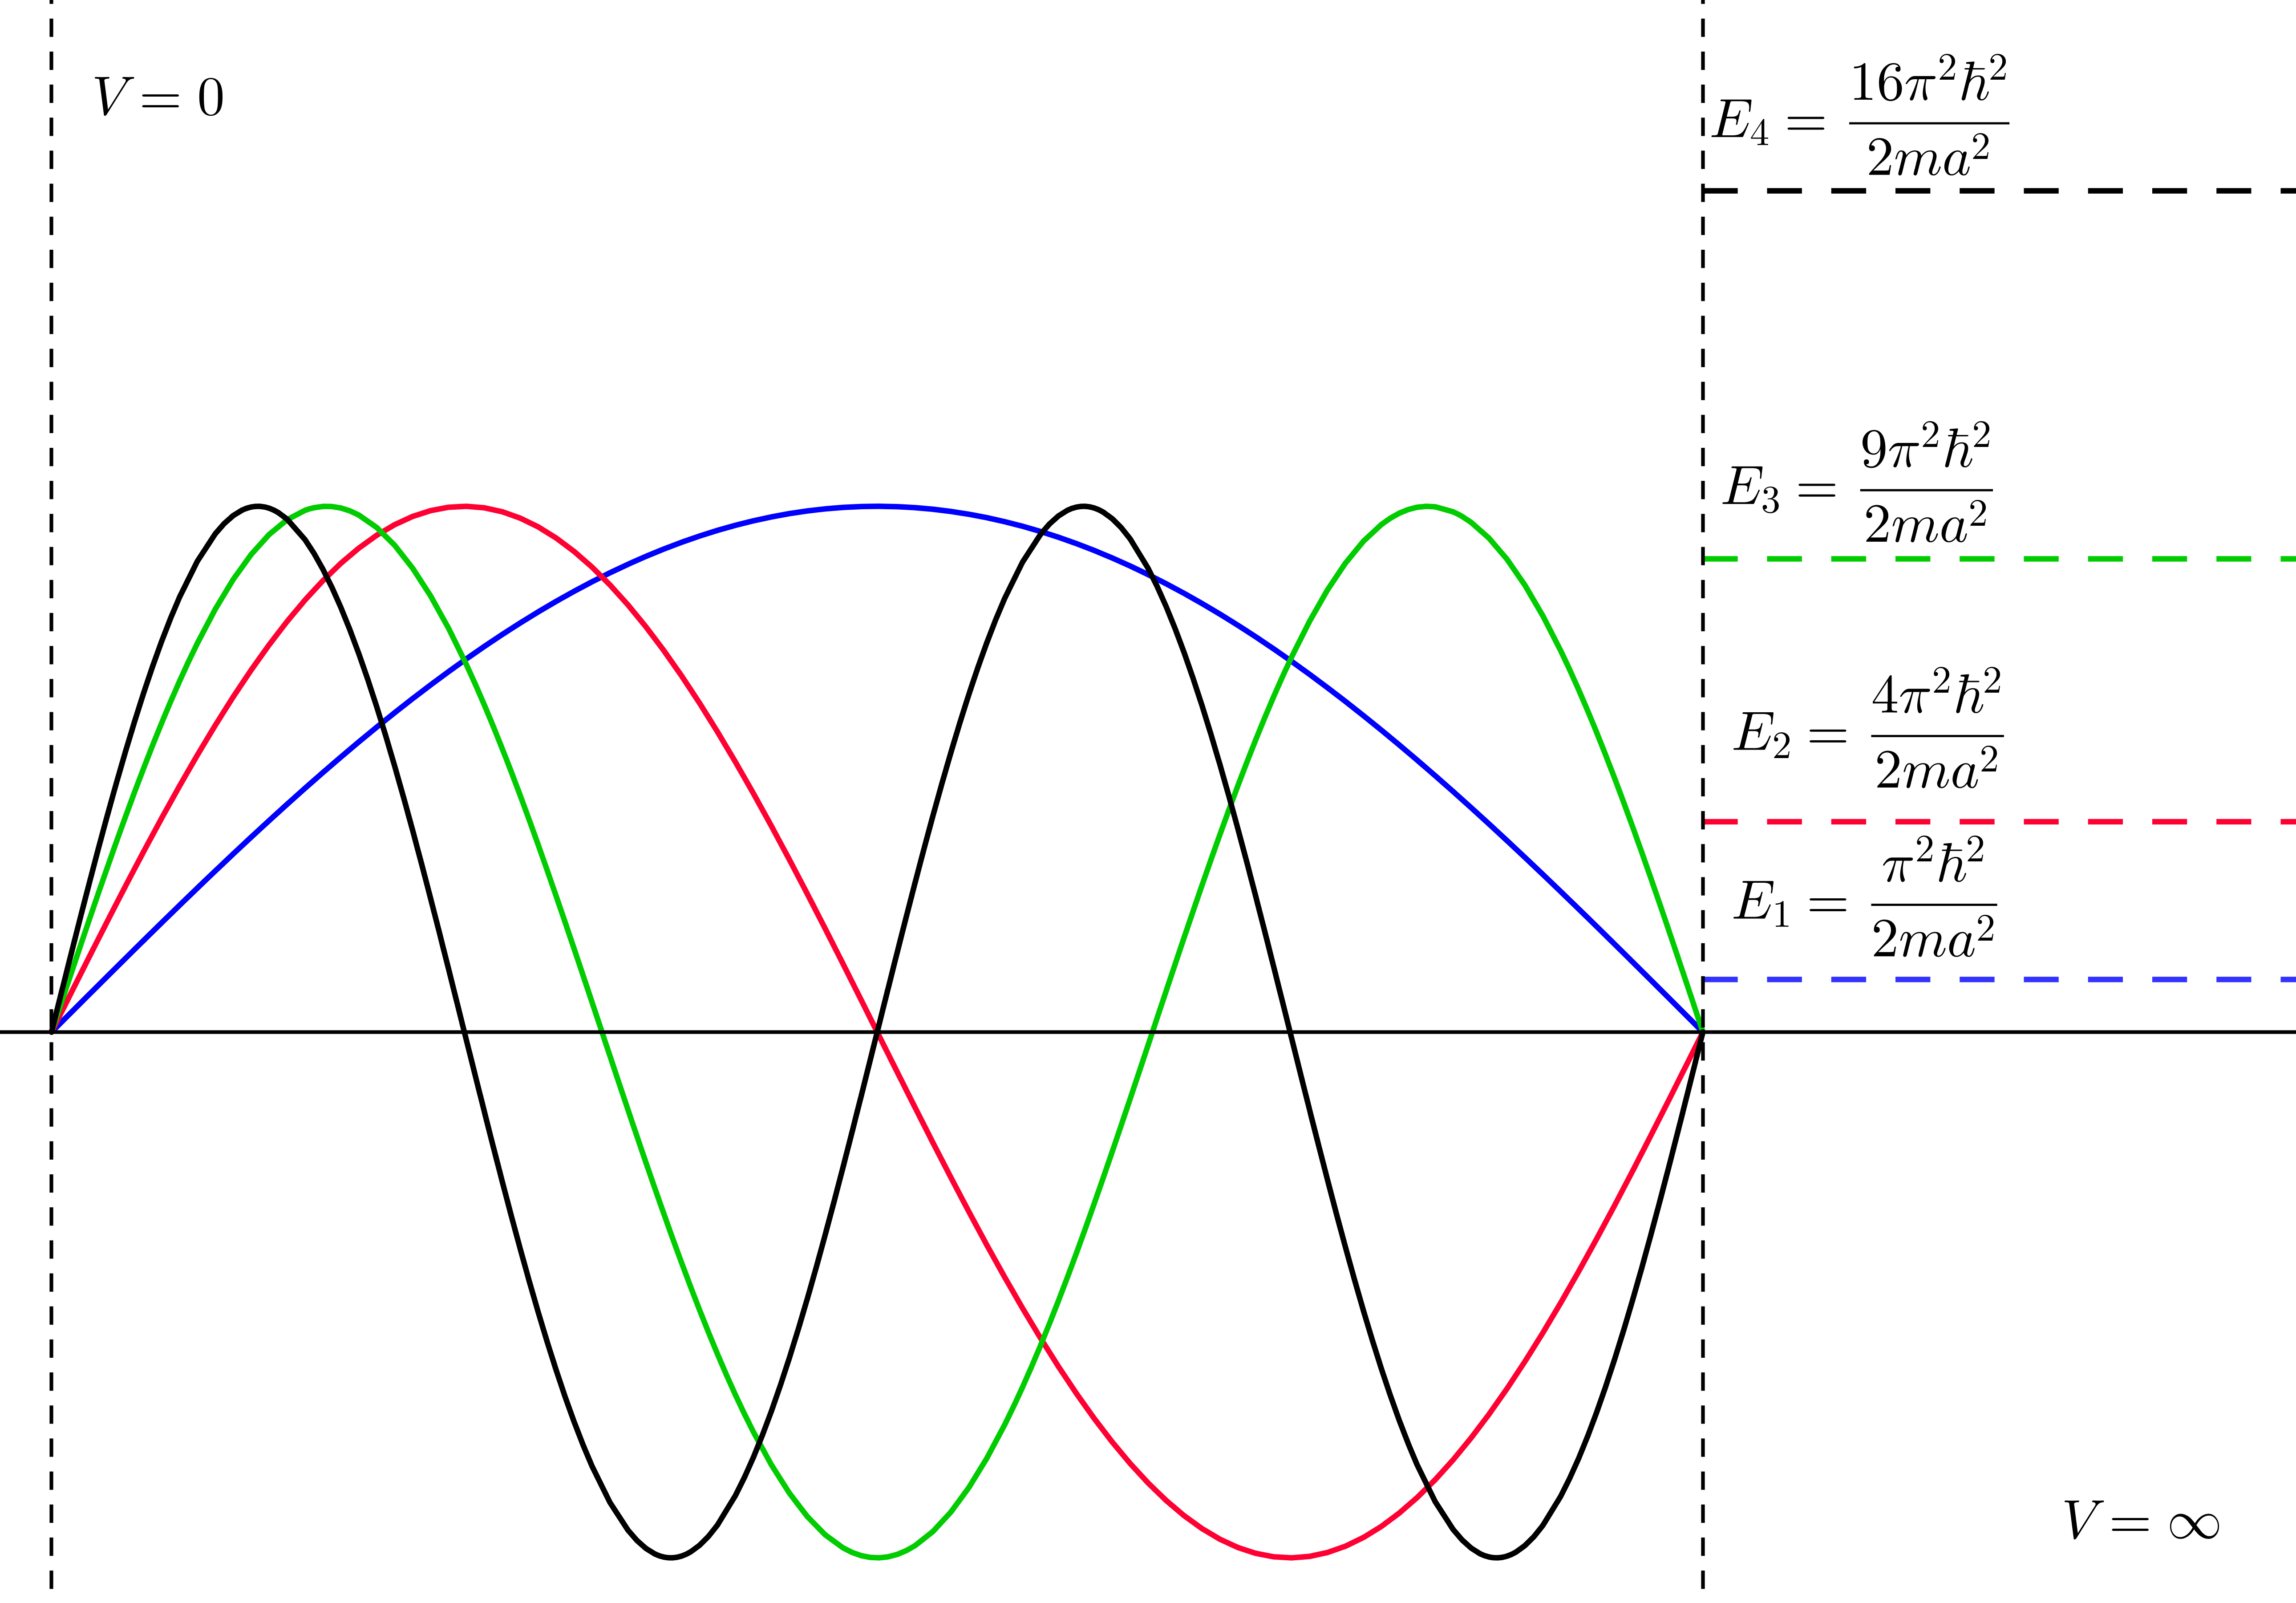
\includegraphics{assets/graphics/1dbox-geo.png}
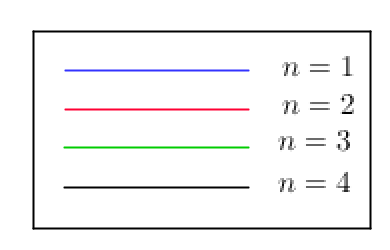
\includegraphics{assets/graphics/n.png}
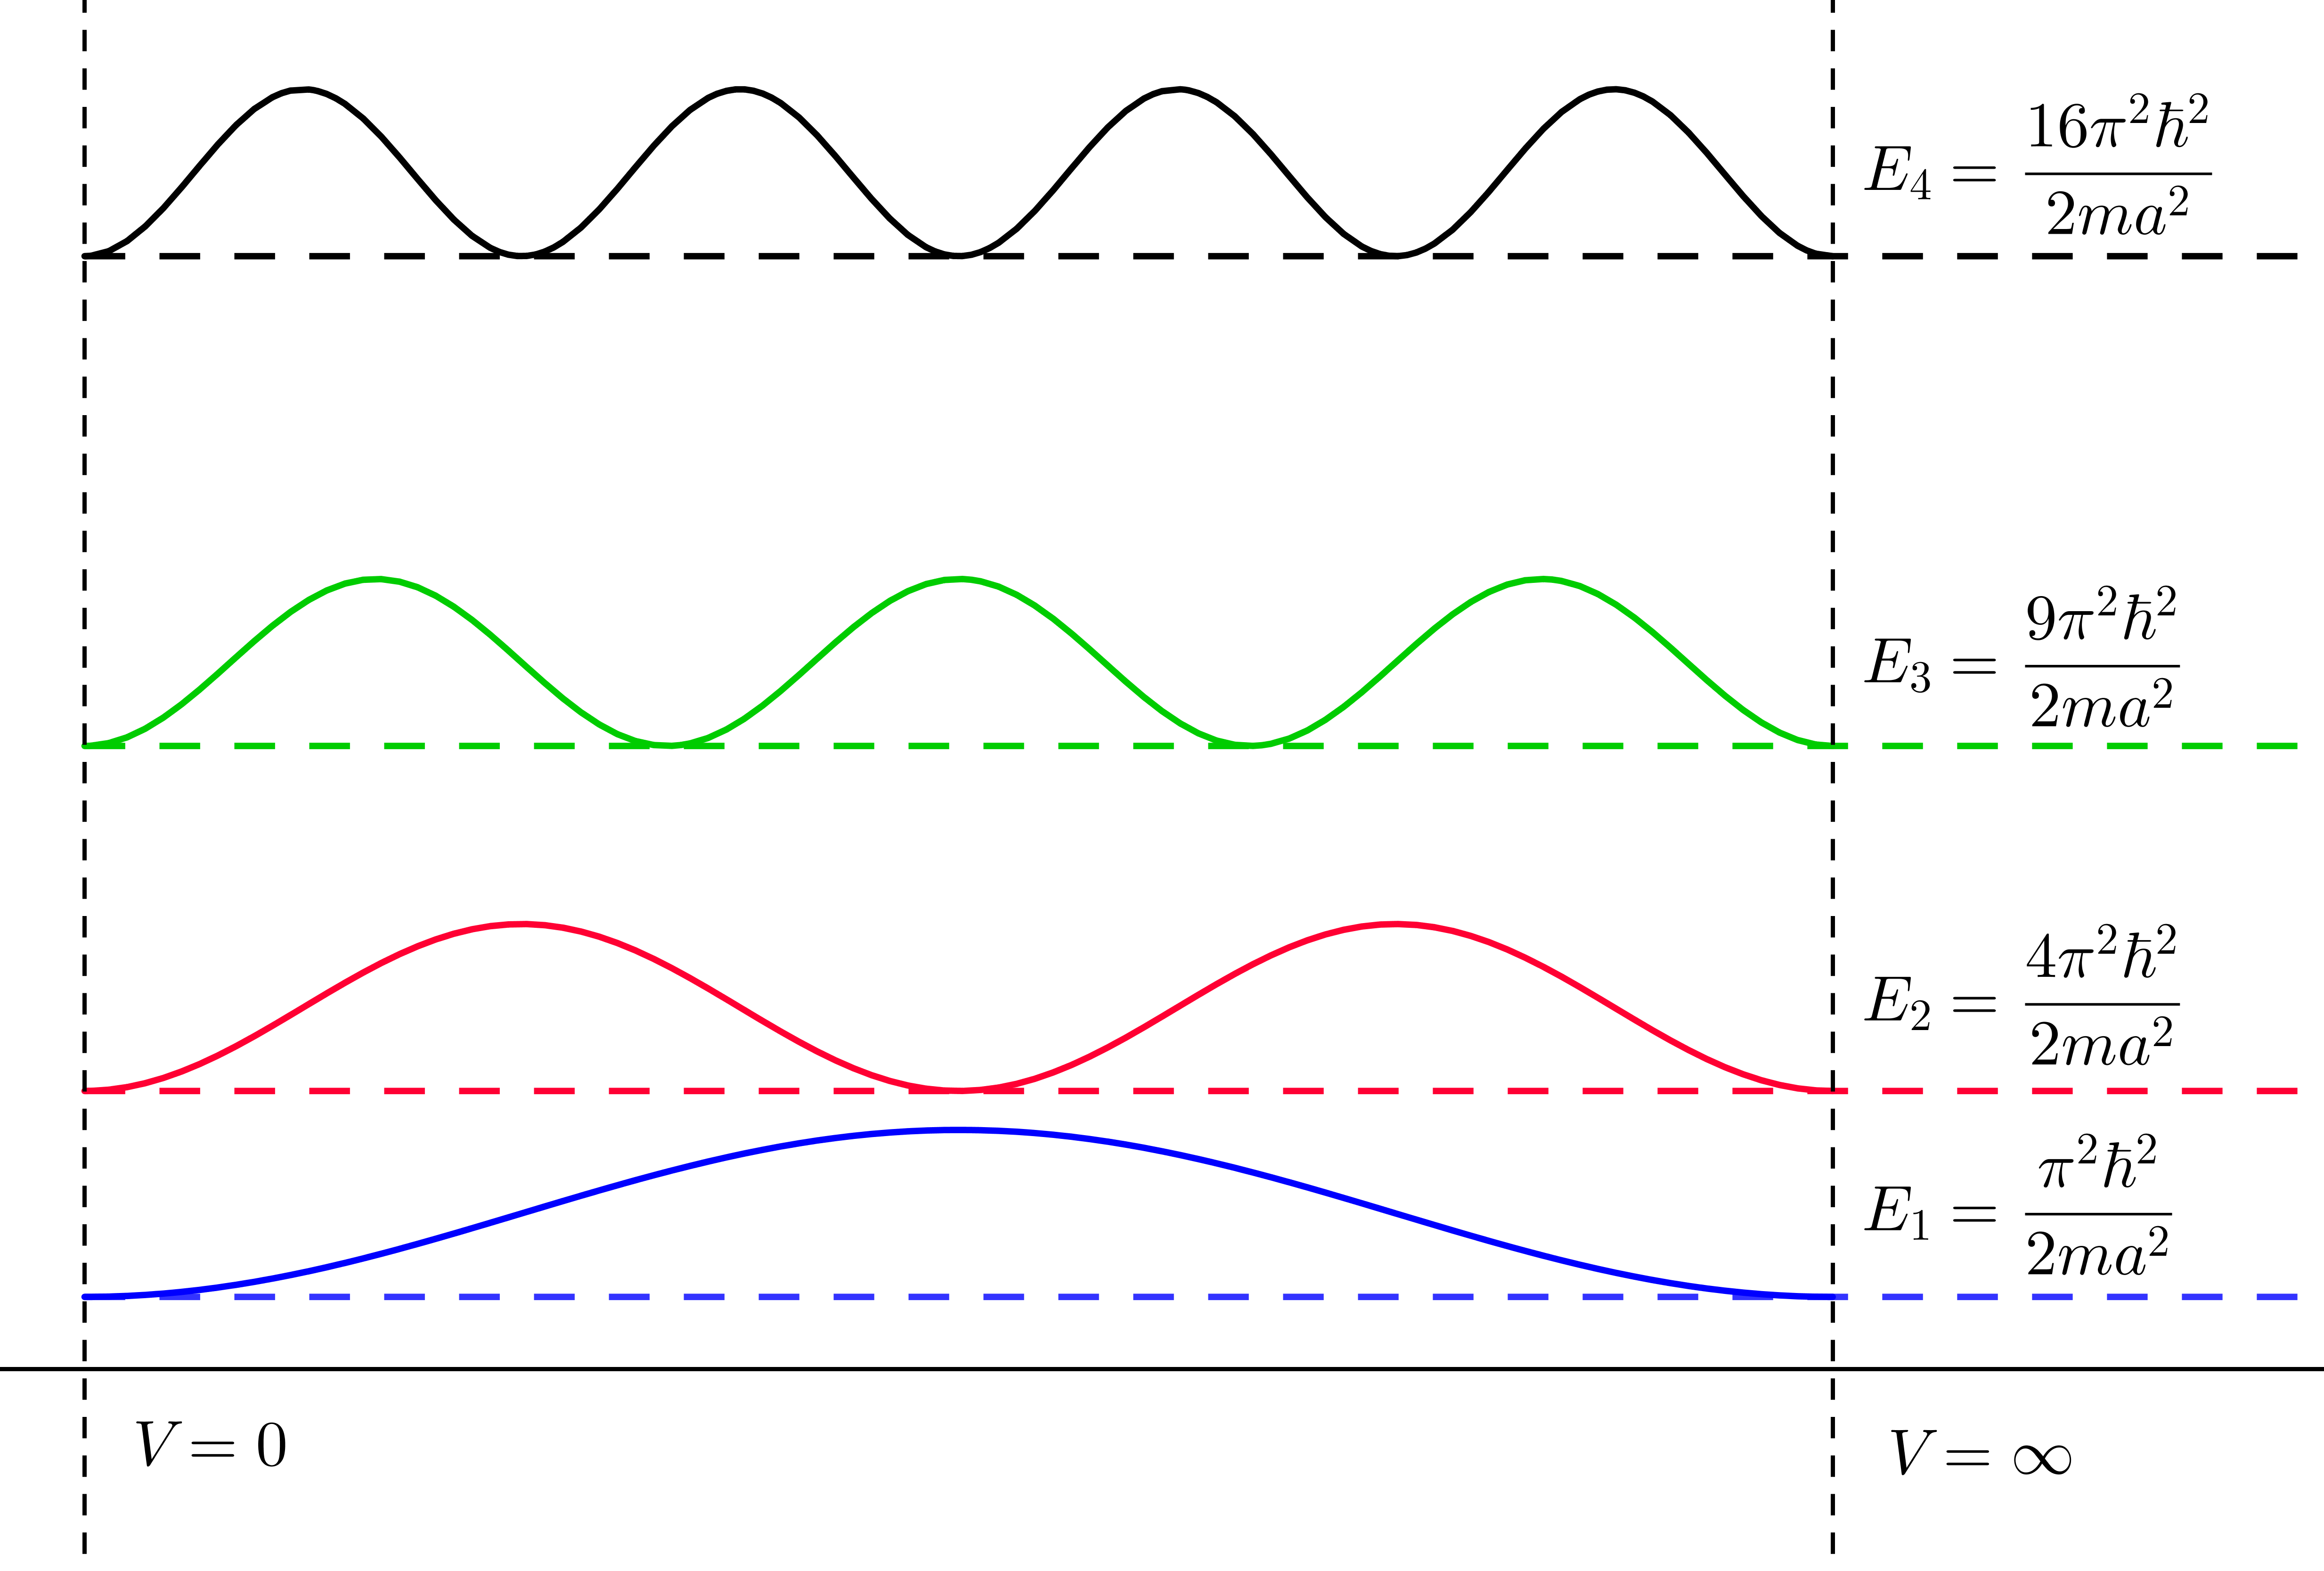
\includegraphics{assets/graphics/1dbox-prob.png}

The wave function should not be interpreted as some sort of function of
space and time. This is a solution to the time-independent Schrödinger
equation and describes a \emph{steady-state}. Recall that the solutions
should be used to generate probability distributions. Then when the
energy corresponds to \(E_i\), \(p:=\rvert\psi_i\rvert^2\) describes the
probability that the particle will be found at a given location.

\section{Particle in a 2-D Box}\label{particle-in-a-2-d-box}

\newcommand{\vecu}{\mathbf{u}}

\newcommand{\ddx}{\frac{d}{dx}}

\section{Discrete Representations}\label{discrete-representations}

At the core of this work is the analogy between discrete and continuous
mathematics --- matrix equations and differential equations. The
time-independent Schrödinger equation
({[}@eq:time\_independent\_schrodinger{]}) is essentially the
second-order differential equation

\begin{equation}H\psi=E\psi \implies -\frac{d^2 }{dx^2}\psi=\lambda \psi\label{eq:second_order_diff_eqn}\end{equation}

generally solved by \(y=\cos \omega x\) and \(y=\sin\omega x\) with
\(\lambda =\omega^2\).

Analogously, we consider the matrix equation (and eigenproblem)

\begin{equation} - D\mathbf{u} = \lambda \mathbf{u}\label{eq:second_difference_eigenproblem}\end{equation}

where \(D\) represents a difference matrix with a specific set of
boundary conditions, \(\mathbf{u}\) is an eigenvector, and \(\lambda\)
is an eigenvalue.

\subsection{\texorpdfstring{Representing a Vector in
\texttt{numpy}}{Representing a Vector in numpy}}\label{representing-a-vector-in-numpy}

It helps to begin to think of this in terms of how we might represent a
function in \texttt{numpy}. Here, we represent the linear function,
\(f(x)=x\) as \(\vecu\) as an evenly spaced vector from 0 to 1 with
steps of \(h=0.1\).

\begin{Shaded}
\begin{Highlighting}[]
\NormalTok{In [}\DecValTok{1}\NormalTok{]: }\ImportTok{import} \NormalTok{numpy}

\NormalTok{In [}\DecValTok{2}\NormalTok{]: u }\OperatorTok{=} \NormalTok{numpy.linspace(}\DecValTok{0}\NormalTok{,}\DecValTok{1}\NormalTok{,}\DecValTok{11}\NormalTok{)}

\NormalTok{In [}\DecValTok{3}\NormalTok{]: u}
\NormalTok{Out[}\DecValTok{3}\NormalTok{]: array([ }\DecValTok{0}\NormalTok{. ,  }\FloatTok{0.1}\NormalTok{,  }\FloatTok{0.2}\NormalTok{,  }\FloatTok{0.3}\NormalTok{,  }\FloatTok{0.4}\NormalTok{,  }\FloatTok{0.5}\NormalTok{,  }\FloatTok{0.6}\NormalTok{,  }\FloatTok{0.7}\NormalTok{,  }\FloatTok{0.8}\NormalTok{,  }\FloatTok{0.9}\NormalTok{,  }\DecValTok{1}\NormalTok{. ])}
\end{Highlighting}
\end{Shaded}

\subsection{Finite Differences}\label{finite-differences}

Consider the derivative:

\begin{equation}f'(x)=\lim_{h\to 0} \frac{f(x+h)-f(x)}{h}\label{eq:first_derivative}\end{equation}

It is not possible to represent a function
\(f: \mathbb{R} \to \mathbb{R}\) computationally because computers are
discrete in nature and require discrete representation. Nor is it
possible to symbolically represent an operation like taking the
derivative. Toward a discrete representation, we consider our function
as a vector and then look at the finite difference method, representing
the derivative as a difference operator.

Toward the difference operator we take

\begin{equation}f'(x)\approx \frac{f(x+h)-f(x)}{h}\label{eq:first_difference}\end{equation}

Recalling that \(\vecu[0]\approx f(0.0)\), \(\vecu[1]\approx f(0.1)\),
\(\vecu[2]\approx f(0.2)\)\dots,

\begin{align*}
\ddx\vecu[0] &= \frac{1}{0.1}\left(\vecu[1] -\vecu[0]\right) = 1\\
\ddx\vecu[1] &= \frac{1}{0.1}\left(\vecu[2] -\vecu[1]\right) = 1\\
\ddx\vecu[2] &= \frac{1}{0.1}\left(\vecu[3] -\vecu[2]\right) = 1\\
&\dots\\
\ddx\vecu[9] &= \frac{1}{0.01}\left(\vecu[10] -\vecu[9]\right) = 1\\
\ddx\vecu[10] &= \frac{1}{0.01}\left(\vecu[11] -\vecu[10]\right) = 1\\
\end{align*}

More generally,

\begin{equation}\frac{d}{dx}\mathbf{u}[x] \approx \frac{1}{h}\left(\mathbf{u}[x+h]-\mathbf{u}[x]\right)=
\frac{1}{h}\left(
\begin{matrix}
1 & -1 &  0 & \dots & 0 & 0 & 0 \\
0 & -1 & 1 & \dots &  0 & 0 & 0 \\
\vdots & \ & \ & \ddots & \ & \ & \vdots \\
0 & 0 & 0 & \dots & 1 & -1 & 0 \\
0 & 0 & 0 & \dots & 0 & 1 & -1 \\
\end{matrix}\right)\mathbf{u}=A \mathbf{u}
\label{eq:first_difference_equation}\end{equation}

Then the first derivative can be approximated by this matrix

\begin{equation}\frac{d}{dx} \approx A = 
\frac{1}{h}\left(\begin{matrix}
1 & -1 &  0 & \dots & 0 & 0 & 0 \\
0 & -1 & 1 & \dots &  0 & 0 & 0 \\
\vdots & \ & \ & \ddots & \ & \ & \vdots \\
0 & 0 & 0 & \dots & 1 & -1 & 0 \\
0 & 0 & 0 & \dots & 0 & 1 & -1 \\
\end{matrix}\right)
\label{eq:first_difference_operator}\end{equation}

\pagebreak

\subsection{Toward Second Difference
Operator}\label{toward-second-difference-operator}

Consider

\begin{align*}
f''(x) &\approx \frac{f'(x+h)-f'(x-h)}{2h}\\
&\approx \frac{\frac{f(x+h)-f(x)}{2h}-\frac{f(x)-f(x-h)}{2h}}{2h}\\
&\approx \frac{f(x+h) - 2f(x) + f(x-h)}{h^2}\tag{with $2h$ recast as $h$}
\end{align*}

\begin{equation}f''(x)\approx \frac{1}{h^2}\left(f(x+h) - 2f(x) + f(x-h)\right)\label{eq:second_difference}\end{equation}

Now consider the following discrete representation

\begin{verbatim}
          |  2 -1  0  0  0  0  0  0  0  0  0 | |0.00| = |-|
          | -1  2 -1  0  0  0  0  0  0  0  0 | |0.01| = |2| 
          |  0 -1  2 -1  0  0  0  0  0  0  0 | |0.04| = |2|
          |  0  0 -1  2 -1  0  0  0  0  0  0 | |0.09| = |2|
          |  0  0  0 -1  2 -1  0  0  0  0  0 | |0.16| = |2|
-1/(.01)  |  0  0  0  0 -1  2 -1  0  0  0  0 | |0.25| = |2|
          |  0  0  0  0  0 -1  2 -1  0  0  0 | |0.36| = |2|
          |  0  0  0  0  0  0 -1  2 -1  0  0 | |0.49| = |2|
          |  0  0  0  0  0  0  0 -1  2 -1  0 | |0.64| = |2|
          |  0  0  0  0  0  0  0  0 -1  2 -1 | |0.81| = |2|
          |  0  0  0  0  0  0  0  0  0 -1  2 | |1.00| = |-|
\end{verbatim}

Note that the vector being multiplied by the matrix corresponds to the
values of \(f(x)=x^2\) at \(x=0.0,0.1,0.2,\dots,0.8,0.9,1.0\). Note that
the matrix is being multiplied by \(\frac{1}{h^2}=\frac{1}{.01}\) where
\(h=0.1\) or the step of our vector representing \(f(x)\). Note that the
returned value is the constant 2 which corresponds to \(f''(x)=2\).

\begin{Shaded}
\begin{Highlighting}[]

\end{Highlighting}
\end{Shaded}

\section{Computational Science}\label{computational-science}

Strang's \emph{Computational Science and Engineering}
{[}@strang2007computational{]} devotes the bulk of its first chapter to
a discussion of this very matrix

\[D =
\frac{1}{h^2}\left(\begin{matrix}
 2 & -1 &  0 & \dots &  0 &  0 &  0 \\
-1 &  2 & -1 & \dots &  0 &  0 &  0 \\
 0 & -1 &  2 & \dots &  0 &  0 &  0 \\
\vdots & \ & \ & \ddots & \ & \ & \vdots \\
 0 &  0 &  0 & \dots &  2 & -1 &  0 \\
 0 &  0 &  0 & \dots & -1 &  2 & -1 \\
 0 &  0 &  0 & \dots &  0 & -1 &  2 \\
\end{matrix}\right)\approx\frac{d^2}{dx^2}
\]

This matrix has several significant properties:

\begin{enumerate}
\def\labelenumi{\arabic{enumi}.}
\tightlist
\item
  It is symmetric.
\item
  It is sparse.
\item
  It is tridiagonal.
\item
  The matrix has constant diagonals.
\item
  It is invertible.
\item
  It is positive
  definite\footnote{This means that the matrix will have $n$ positive (and therefore real) eigenvalues. From this we know that the matrix $D$ is self-adjoint.}.
\end{enumerate}

\subsection{Numpy and Scipy as Wrapper to BLAS and
Lapack}\label{numpy-and-scipy-as-wrapper-to-blas-and-lapack}

If performance is a priority than computational mathematics must be done
using C and its libraries \href{http://www.netlib.org/blas/}{BLAS},
\href{http://www.netlib.org/lapack/}{Lapack}, and
\href{http://www.caam.rice.edu/software/ARPACK/}{Arpack}. Prior to
understanding the underlying mathematics, we posit that rapid
prototyping and an interactive development environment should be
prioritized over performance. Toward this end, we offer as an
alternative to C and its computational libraries, Python and its
computational libraries \href{http://www.numpy.org/}{Numpy} and
\href{http://www.scipy.org/}{Scipy}. Numpy and Scipy are open-source
(free in all senses). Numpy and Scipy offer a robust interactive
development environment in \href{http://ipython.org/}{IPython}.
Furthermore, we believe that Python syntax is descended from C syntax
and note that Numpy and Scipy are high-level wrappers to the same
Fortran functions being used in BLAS and Lapack, and therefore porting a
robust and vetted algorithm from Python to C should be straight-forward
where non-trivial.

Later in this document we explore the
\href{https://www.gnu.org/software/gsl/}{Gnu Scientific Library}.

Worth further invesigation are going directly to netlib which is largely
maintained in Fortran. Netlib maintains
\href{http://www.netlib.org/blas/}{BLAS},
\href{http://www.netlib.org/lapack/}{LAPACK},
\href{http://icl.cs.utk.edu/plasma/}{PLASMA}, and
\href{http://icl.cs.utk.edu/magma/}{MAGMA}.

\vfill

\pagebreak

\subsection{Implementing a Second Difference Matrix in
numpy}\label{implementing-a-second-difference-matrix-in-numpy}

We have written the following function based upon \emph{CSE}
{[}@strang2007computational{]}. It creates four matrices, each
corresponding to a different set of boundary conditions: \texttt{D}, for
Dirichlet\footnote{Also known as \emph{fixed-fixed conditions} and defined by zeroes at the boundaries of the function.},
\texttt{R} for
Robin\footnote{Also known as \emph{free-fixed conditions} and defined by zero in the first derivative of the function at one end of the function and zero in the value of the function at the other.},
\texttt{N} for
Neuman\footnote{Also known as \emph{free-free conditions} and defined by zeroes in the first derivative of the function at the boundaries of the function.},
or \texttt{C} for
circular\footnote{Defined by equality in the value of the function and in the value of its first derivative at the boundaries}.

\begin{Shaded}
\begin{Highlighting}[]
\KeywordTok{def} \NormalTok{secondDiff(}\BuiltInTok{type}\NormalTok{,n}\OperatorTok{=}\DecValTok{10}\NormalTok{,sparse}\OperatorTok{=}\VariableTok{False}\NormalTok{):}
    \CommentTok{'''}
\CommentTok{    secondDiff Create finite difference model matrix.}
\CommentTok{    TYPE is one of the characters 'D', 'R', 'N', or 'C'.}
\CommentTok{    3rd argument is boolean for sparseness}
\CommentTok{    '''}
    \ImportTok{import} \NormalTok{numpy, scipy.sparse}
    \NormalTok{e }\OperatorTok{=} \NormalTok{numpy.ones(n)}
    \NormalTok{e_off }\OperatorTok{=} \NormalTok{numpy.ones(n}\DecValTok{-1}\NormalTok{)}
    \NormalTok{D }\OperatorTok{=} \NormalTok{scipy.sparse.csr_matrix(}
      \NormalTok{scipy.sparse.diags([e_off,}\OperatorTok{-}\DecValTok{2}\OperatorTok{*}\NormalTok{e,e_off],[}\OperatorTok{-}\DecValTok{1}\NormalTok{,}\DecValTok{0}\NormalTok{,}\DecValTok{1}\NormalTok{]))}

    \ControlFlowTok{if} \NormalTok{(}\BuiltInTok{str}\NormalTok{(}\BuiltInTok{type}\NormalTok{) }\OperatorTok{==} \StringTok{'R'} \OperatorTok{or} \BuiltInTok{str}\NormalTok{(}\BuiltInTok{type}\NormalTok{) }\OperatorTok{==} \StringTok{'T'} \OperatorTok{or}
        \BuiltInTok{str}\NormalTok{(}\BuiltInTok{type}\NormalTok{) }\OperatorTok{==} \StringTok{'N'} \OperatorTok{or} \BuiltInTok{str}\NormalTok{(}\BuiltInTok{type}\NormalTok{) }\OperatorTok{==} \StringTok{'B'}\NormalTok{):}
        \NormalTok{D[}\DecValTok{0}\NormalTok{,}\DecValTok{0}\NormalTok{] }\OperatorTok{=} \OperatorTok{-}\DecValTok{1}
    \ControlFlowTok{if} \NormalTok{(}\BuiltInTok{str}\NormalTok{(}\BuiltInTok{type}\NormalTok{) }\OperatorTok{==} \StringTok{'N'} \OperatorTok{or} \BuiltInTok{str}\NormalTok{(}\BuiltInTok{type}\NormalTok{) }\OperatorTok{==} \StringTok{'B'}\NormalTok{):}
        \NormalTok{D[n}\DecValTok{-1}\NormalTok{,n}\DecValTok{-1}\NormalTok{] }\OperatorTok{=} \OperatorTok{-}\DecValTok{1}
    \ControlFlowTok{if} \BuiltInTok{str}\NormalTok{(}\BuiltInTok{type}\NormalTok{) }\OperatorTok{==} \StringTok{'C'}\NormalTok{:}
        \NormalTok{D[}\DecValTok{0}\NormalTok{,n}\DecValTok{-1}\NormalTok{] }\OperatorTok{=} \DecValTok{1}
        \NormalTok{D[n}\DecValTok{-1}\NormalTok{,}\DecValTok{0}\NormalTok{] }\OperatorTok{=} \DecValTok{1}

    \ControlFlowTok{if} \NormalTok{sparse }\OperatorTok{==} \VariableTok{False}\NormalTok{: }\ControlFlowTok{return} \NormalTok{D.todense()}
    \ControlFlowTok{else}\NormalTok{: }\ControlFlowTok{return} \NormalTok{D}
\end{Highlighting}
\end{Shaded}

\vfill

\pagebreak

\vfill

\pagebreak

\subsection{Discrete Representation of the Particle in a
Box}\label{discrete-representation-of-the-particle-in-a-box}

To conclude this introduction, we note that we can discretely represent
the Hamiltonian operator ({[}@eq:hamiltonian\_particle\_in\_a\_box{]})
describing the ``particle in a box'' using the matrix \texttt{D} defined
by this function.

We use the IPython interactive terminal to execute the commands and find
its \texttt{\%paste} magic function very useful.

We first load the function \texttt{secondDiff}.

We then load the following python modules:

\begin{Shaded}
\begin{Highlighting}[]
\NormalTok{In [}\DecValTok{2}\NormalTok{]: }\ImportTok{import} \NormalTok{numpy, numpy.linalg, scipy.linalg, matplotlib.pyplot}

\CommentTok{## -- End pasted test --}
\end{Highlighting}
\end{Shaded}

We define the matrix equation describing the particle in a box as

\begin{equation}-D\mathbf{u}=\frac{2mE}{\hbar^2} \mathbf{u}\label{eq:matrix_eqn_particle_in_a_box}\end{equation}

For \(D\), which describes Dirichlet boundary conditions, we have

\begin{itemize}
\tightlist
\item
  \(\theta_k = k\pi/(n+1)\)
\item
  eigenvalues, \(E_k = 2-2\cos\theta_k\)
\item
  eigenfunctions,
  \(u_k = (\sin k\pi h, \sin 2k\pi h, \dots, \sin n\pi h)\)
\end{itemize}

for \(k\in[1,n]\).

We define each of these in our IPython session.

\vfill

\pagebreak

\begin{Shaded}
\begin{Highlighting}[]
\NormalTok{In [}\DecValTok{3}\NormalTok{]: }\OperatorTok{%}\NormalTok{paste}
\KeywordTok{def} \NormalTok{K_theta(k,n):}
  \ControlFlowTok{return} \NormalTok{k}\OperatorTok{*}\NormalTok{numpy.pi}\OperatorTok{/}\NormalTok{(n}\DecValTok{+1}\NormalTok{)}

\KeywordTok{def} \NormalTok{K_eigenvalues(n):}
  \ControlFlowTok{return} \DecValTok{2}\OperatorTok{*}\NormalTok{numpy.ones(n) }\OperatorTok{-} \DecValTok{2}\OperatorTok{*}\NormalTok{numpy.cos(K_theta(numpy.linspace(n,}\DecValTok{1}\NormalTok{,n),n))}

\KeywordTok{def} \NormalTok{K_eigenfunction(k,n):}
  \NormalTok{vec }\OperatorTok{=} \NormalTok{numpy.sin(K_theta(numpy.linspace(}\DecValTok{1}\NormalTok{,n,n),n)}\OperatorTok{*}\NormalTok{k)}
  \ControlFlowTok{return} \NormalTok{vec}\OperatorTok{/}\NormalTok{numpy.linalg.norm(vec)}

\CommentTok{## -- End pasted text --}
\end{Highlighting}
\end{Shaded}

We next create our second difference matrices for Dirichlet boundary
conditions with \(n=2,3,4,5\). We display \texttt{K4} for visual
inspection.

\begin{Shaded}
\begin{Highlighting}[]
\NormalTok{In [}\DecValTok{4}\NormalTok{]: }\OperatorTok{%}\NormalTok{paste}
\NormalTok{K2 }\OperatorTok{=} \OperatorTok{-}\NormalTok{secondDiff(}\StringTok{'D'}\NormalTok{,}\DecValTok{2}\NormalTok{)}
\NormalTok{K3 }\OperatorTok{=} \OperatorTok{-}\NormalTok{secondDiff(}\StringTok{'D'}\NormalTok{,}\DecValTok{3}\NormalTok{)}
\NormalTok{K4 }\OperatorTok{=} \OperatorTok{-}\NormalTok{secondDiff(}\StringTok{'D'}\NormalTok{,}\DecValTok{4}\NormalTok{)}
\NormalTok{K5 }\OperatorTok{=} \OperatorTok{-}\NormalTok{secondDiff(}\StringTok{'D'}\NormalTok{,}\DecValTok{5}\NormalTok{)}
\BuiltInTok{print} \NormalTok{K4}

\CommentTok{## -- End pasted text --}
\NormalTok{[[ }\DecValTok{2}\NormalTok{. }\OperatorTok{-}\DecValTok{1}\NormalTok{. }\OperatorTok{-}\DecValTok{0}\NormalTok{. }\OperatorTok{-}\DecValTok{0}\NormalTok{.]}
 \NormalTok{[}\OperatorTok{-}\DecValTok{1}\NormalTok{.  }\DecValTok{2}\NormalTok{. }\OperatorTok{-}\DecValTok{1}\NormalTok{. }\OperatorTok{-}\DecValTok{0}\NormalTok{.]}
 \NormalTok{[}\OperatorTok{-}\DecValTok{0}\NormalTok{. }\OperatorTok{-}\DecValTok{1}\NormalTok{.  }\DecValTok{2}\NormalTok{. }\OperatorTok{-}\DecValTok{1}\NormalTok{.]}
 \NormalTok{[}\OperatorTok{-}\DecValTok{0}\NormalTok{. }\OperatorTok{-}\DecValTok{0}\NormalTok{. }\OperatorTok{-}\DecValTok{1}\NormalTok{.  }\DecValTok{2}\NormalTok{.]]}
\end{Highlighting}
\end{Shaded}

\vfill

\pagebreak

\subsection{Finding Eigenvalues}\label{finding-eigenvalues}

We then use the built-in eigensolver in \texttt{numpy.linalg} to find
the eigenvalues and compare it to the values generated by our function.
Note that the first element in the array returned by
\texttt{numpy.linalg.eig} is an array of the eigenvalues.

\begin{Shaded}
\begin{Highlighting}[]
\NormalTok{In [}\DecValTok{5}\NormalTok{]: }\OperatorTok{%}\NormalTok{paste}
\NormalTok{e2 }\OperatorTok{=} \NormalTok{numpy.linalg.eig(K2)}
\NormalTok{e3 }\OperatorTok{=} \NormalTok{numpy.linalg.eig(K3)}
\NormalTok{e4 }\OperatorTok{=} \NormalTok{numpy.linalg.eig(K4)}
\NormalTok{e5 }\OperatorTok{=} \NormalTok{numpy.linalg.eig(K5)}
\BuiltInTok{print} \NormalTok{e2[}\DecValTok{0}\NormalTok{]}
\BuiltInTok{print} \NormalTok{K_eigenvalues(}\DecValTok{2}\NormalTok{)}
\BuiltInTok{print} \NormalTok{e3[}\DecValTok{0}\NormalTok{]}
\BuiltInTok{print} \NormalTok{K_eigenvalues(}\DecValTok{3}\NormalTok{)}
\BuiltInTok{print} \NormalTok{e4[}\DecValTok{0}\NormalTok{]}
\BuiltInTok{print} \NormalTok{K_eigenvalues(}\DecValTok{4}\NormalTok{)}
\BuiltInTok{print} \NormalTok{e5[}\DecValTok{0}\NormalTok{]}
\BuiltInTok{print} \NormalTok{K_eigenvalues(}\DecValTok{5}\NormalTok{)}

\CommentTok{## -- End pasted text --}
\NormalTok{[ }\DecValTok{3}\NormalTok{.  }\DecValTok{1}\NormalTok{.]}
\NormalTok{[ }\DecValTok{3}\NormalTok{.  }\DecValTok{1}\NormalTok{.]}
\NormalTok{[ }\FloatTok{3.41421356}  \DecValTok{2}\NormalTok{.          }\FloatTok{0.58578644}\NormalTok{]}
\NormalTok{[ }\FloatTok{3.41421356}  \DecValTok{2}\NormalTok{.          }\FloatTok{0.58578644}\NormalTok{]}
\NormalTok{[ }\FloatTok{3.61803399}  \FloatTok{2.61803399}  \FloatTok{0.38196601}  \FloatTok{1.38196601}\NormalTok{]}
\NormalTok{[ }\FloatTok{3.61803399}  \FloatTok{2.61803399}  \FloatTok{1.38196601}  \FloatTok{0.38196601}\NormalTok{]}
\NormalTok{[ }\FloatTok{3.73205081}  \DecValTok{3}\NormalTok{.          }\DecValTok{2}\NormalTok{.          }\FloatTok{0.26794919}  \DecValTok{1}\NormalTok{.        ]}
\NormalTok{[ }\FloatTok{3.73205081}  \DecValTok{3}\NormalTok{.          }\DecValTok{2}\NormalTok{.          }\DecValTok{1}\NormalTok{.          }\FloatTok{0.26794919}\NormalTok{]}
\end{Highlighting}
\end{Shaded}

\vfill

\pagebreak

\subsection{Finding Eigenvectors}\label{finding-eigenvectors}

The second element in the array by \texttt{numpy.linalg.eig} is a matrix
of the eigenfunctions. Please understand that we are liberal with our
implicit understanding that eigenfunctions and eigenvectors are, for our
purposes, synonymous.

\begin{Shaded}
\begin{Highlighting}[]
\NormalTok{In [}\DecValTok{6}\NormalTok{]: }\OperatorTok{%}\NormalTok{paste}
\BuiltInTok{print} \NormalTok{e2[}\DecValTok{1}\NormalTok{]}
\BuiltInTok{print} \NormalTok{K_eigenfunction(}\DecValTok{1}\NormalTok{,}\DecValTok{2}\NormalTok{)}
\BuiltInTok{print} \NormalTok{K_eigenfunction(}\DecValTok{2}\NormalTok{,}\DecValTok{2}\NormalTok{)}

\CommentTok{## -- End pasted text --}
\NormalTok{[[ }\FloatTok{0.70710678}  \FloatTok{0.70710678}\NormalTok{]}
 \NormalTok{[}\OperatorTok{-}\FloatTok{0.70710678}  \FloatTok{0.70710678}\NormalTok{]]}
\NormalTok{[ }\FloatTok{0.70710678}  \FloatTok{0.70710678}\NormalTok{]}
\NormalTok{[ }\FloatTok{0.70710678} \OperatorTok{-}\FloatTok{0.70710678}\NormalTok{]}

\NormalTok{In [}\DecValTok{7}\NormalTok{]: }\OperatorTok{%}\NormalTok{paste}
\BuiltInTok{print} \NormalTok{e4[}\DecValTok{1}\NormalTok{]}
\BuiltInTok{print} \NormalTok{K_eigenfunction(}\DecValTok{1}\NormalTok{,}\DecValTok{4}\NormalTok{)}
\BuiltInTok{print} \NormalTok{K_eigenfunction(}\DecValTok{2}\NormalTok{,}\DecValTok{4}\NormalTok{)}
\BuiltInTok{print} \NormalTok{K_eigenfunction(}\DecValTok{3}\NormalTok{,}\DecValTok{4}\NormalTok{)}
\BuiltInTok{print} \NormalTok{K_eigenfunction(}\DecValTok{4}\NormalTok{,}\DecValTok{4}\NormalTok{)}

\CommentTok{## -- End pasted text --}
\NormalTok{[[}\OperatorTok{-}\FloatTok{0.37174803} \OperatorTok{-}\FloatTok{0.60150096} \OperatorTok{-}\FloatTok{0.37174803} \OperatorTok{-}\FloatTok{0.60150096}\NormalTok{]}
 \NormalTok{[ }\FloatTok{0.60150096}  \FloatTok{0.37174803} \OperatorTok{-}\FloatTok{0.60150096} \OperatorTok{-}\FloatTok{0.37174803}\NormalTok{]}
 \NormalTok{[}\OperatorTok{-}\FloatTok{0.60150096}  \FloatTok{0.37174803} \OperatorTok{-}\FloatTok{0.60150096}  \FloatTok{0.37174803}\NormalTok{]}
 \NormalTok{[ }\FloatTok{0.37174803} \OperatorTok{-}\FloatTok{0.60150096} \OperatorTok{-}\FloatTok{0.37174803}  \FloatTok{0.60150096}\NormalTok{]]}
\NormalTok{[ }\FloatTok{0.37174803}  \FloatTok{0.60150096}  \FloatTok{0.60150096}  \FloatTok{0.37174803}\NormalTok{]}
\NormalTok{[ }\FloatTok{0.60150096}  \FloatTok{0.37174803} \OperatorTok{-}\FloatTok{0.37174803} \OperatorTok{-}\FloatTok{0.60150096}\NormalTok{]}
\NormalTok{[ }\FloatTok{0.60150096} \OperatorTok{-}\FloatTok{0.37174803} \OperatorTok{-}\FloatTok{0.37174803}  \FloatTok{0.60150096}\NormalTok{]}
\NormalTok{[ }\FloatTok{0.37174803} \OperatorTok{-}\FloatTok{0.60150096}  \FloatTok{0.60150096} \OperatorTok{-}\FloatTok{0.37174803}\NormalTok{]}
\end{Highlighting}
\end{Shaded}

\subsection{Comparison of timing}\label{comparison-of-timing}

For comparison of timing, we introduce a function that will return the
exact same values as the built-in eigensolver.

\begin{Shaded}
\begin{Highlighting}[]
\NormalTok{In [}\DecValTok{8}\NormalTok{]: }\OperatorTok{%}\NormalTok{paste}
\KeywordTok{def} \NormalTok{my_eig(n):}
    \NormalTok{vals }\OperatorTok{=} \NormalTok{[]}
    \NormalTok{vals.append(K_eigenvalues(n))}
    \NormalTok{eigenvectors }\OperatorTok{=} \NormalTok{numpy.matrix(K_eigenfunction(}\DecValTok{1}\NormalTok{,n))}
    \ControlFlowTok{for} \NormalTok{i }\OperatorTok{in} \BuiltInTok{range}\NormalTok{(n}\DecValTok{-1}\NormalTok{):}
        \NormalTok{eigenvectors }\OperatorTok{=} \NormalTok{numpy.r_[eigenvectors,}
                                \NormalTok{numpy.matrix(K_eigenfunction(i}\DecValTok{+2}\NormalTok{,n))]}
    \NormalTok{vals.append(eigenvectors)}
    \ControlFlowTok{return} \NormalTok{vals}

\CommentTok{## -- End pasted text --}
\end{Highlighting}
\end{Shaded}

We visually inspect the three by three output.

\begin{Shaded}
\begin{Highlighting}[]
\NormalTok{In [}\DecValTok{9}\NormalTok{]: }\OperatorTok{%}\NormalTok{paste}
\BuiltInTok{print} \NormalTok{my_eig(}\DecValTok{3}\NormalTok{)}
\BuiltInTok{print} \NormalTok{numpy.linalg.eig(K3)}

\CommentTok{## -- End pasted text --}
\NormalTok{[array([ }\FloatTok{3.41421356}\NormalTok{,  }\DecValTok{2}\NormalTok{.        ,  }\FloatTok{0.58578644}\NormalTok{]),}
\NormalTok{matrix([[  }\FloatTok{5.00000000e-01}\NormalTok{,   }\FloatTok{7.07106781e-01}\NormalTok{,   }\FloatTok{5.00000000e-01}\NormalTok{],}
        \NormalTok{[  }\FloatTok{7.07106781e-01}\NormalTok{,   }\FloatTok{8.65956056e-17}\NormalTok{,  }\OperatorTok{-}\FloatTok{7.07106781e-01}\NormalTok{],}
        \NormalTok{[  }\FloatTok{5.00000000e-01}\NormalTok{,  }\OperatorTok{-}\FloatTok{7.07106781e-01}\NormalTok{,   }\FloatTok{5.00000000e-01}\NormalTok{]])]}
\NormalTok{(array([ }\FloatTok{3.41421356}\NormalTok{,  }\DecValTok{2}\NormalTok{.        ,  }\FloatTok{0.58578644}\NormalTok{]),}
\NormalTok{matrix([[ }\OperatorTok{-}\FloatTok{5.00000000e-01}\NormalTok{,  }\OperatorTok{-}\FloatTok{7.07106781e-01}\NormalTok{,   }\FloatTok{5.00000000e-01}\NormalTok{],}
        \NormalTok{[  }\FloatTok{7.07106781e-01}\NormalTok{,   }\FloatTok{4.05925293e-16}\NormalTok{,   }\FloatTok{7.07106781e-01}\NormalTok{],}
        \NormalTok{[ }\OperatorTok{-}\FloatTok{5.00000000e-01}\NormalTok{,   }\FloatTok{7.07106781e-01}\NormalTok{,   }\FloatTok{5.00000000e-01}\NormalTok{]]))}
\end{Highlighting}
\end{Shaded}

\vfill

\pagebreak

We use the IPython magic function \texttt{\%timeit} to run our timing
comparisons.

\begin{Shaded}
\begin{Highlighting}[]
\NormalTok{In [}\DecValTok{10}\NormalTok{]: }\OperatorTok\NormalTok{timeit numpy.linalg.eig(K5)}
\OperatorTok{%}\NormalTok{timeit my_eig(}\DecValTok{5}\NormalTok{)}

\CommentTok{## -- End pasted text --}
\NormalTok{The slowest run took }\FloatTok{6.73} \NormalTok{times longer than the fastest.}
\NormalTok{This could mean that an intermediate result }\OperatorTok{is} \NormalTok{being cached}
\DecValTok{10000} \NormalTok{loops, best of }\DecValTok{3}\NormalTok{: }\FloatTok{31.8} \NormalTok{µs per loop}
\DecValTok{1000} \NormalTok{loops, best of }\DecValTok{3}\NormalTok{: }\DecValTok{188} \NormalTok{µs per loop}
\end{Highlighting}
\end{Shaded}

We note that the built-in eigensolver is nearly six times faster than
our algorithm.

\begin{Shaded}
\begin{Highlighting}[]
\NormalTok{In [}\DecValTok{11}\NormalTok{]: }\OperatorTok\NormalTok{timeit numpy.linalg.eig(K10)}
\OperatorTok{%}\NormalTok{timeit my_eig(}\DecValTok{10}\NormalTok{)}

\CommentTok{## -- End pasted text --}
\DecValTok{10000} \NormalTok{loops, best of }\DecValTok{3}\NormalTok{: }\FloatTok{49.8} \NormalTok{µs per loop}
\DecValTok{1000} \NormalTok{loops, best of }\DecValTok{3}\NormalTok{: }\DecValTok{427} \NormalTok{µs per loop}
\end{Highlighting}
\end{Shaded}

We note that the built-in eigensolver is nearly ten times faster than
our algorithm.

\begin{Shaded}
\begin{Highlighting}[]
\NormalTok{In [}\DecValTok{12}\NormalTok{]: }\OperatorTok\NormalTok{timeit numpy.linalg.eig(K100)}
\OperatorTok{%}\NormalTok{timeit my_eig(}\DecValTok{100}\NormalTok{)}

\CommentTok{## -- End pasted text --}
\DecValTok{100} \NormalTok{loops, best of }\DecValTok{3}\NormalTok{: }\FloatTok{9.06} \NormalTok{ms per loop}
\DecValTok{100} \NormalTok{loops, best of }\DecValTok{3}\NormalTok{: }\FloatTok{4.97} \NormalTok{ms per loop}
\end{Highlighting}
\end{Shaded}

This last result is astounding. Suddenly our algorithm is almost twice
as fast as the built-in solver.

\vfill

\pagebreak

\subsection{Exploring This Result}\label{exploring-this-result}

We wish to collect data over times to find eigenvalues and eigenvectors
for increasing values of \(n\). Note that our method does not actually
use the matrix, but rather uses analytical results based on our
knowledge of the second difference matrix for Dirichlet boundary
conditions. We will need, however, to pass a matrix to the built-in
eigensolver. We wish to create this matrix outside of the timer so as
not to penalize the eigensolver.

We wrote the following simple IPython script:

\begin{verbatim}
for i in range(3,300):
    matrix = secondDiff('D',n)
    result_my  = %timeit -o my_eig(n)
    result_sys = %timeit -o numpy.linalg.eig(matrix)
    %store result_my.best, result_sys.best >> output.txt


import numpy, numpy.linalg, matplotlib.pyplot
data = numpy.genfromtxt('output_1442991327.csv', delimiter=',')
indep = data[:,0]
my_eig_data = data[:,1]
sys_eig_data = data[:,2]
my_eigensolver = matplotlib.pyplot.plot(indep,my_eig_data)
system_eigensolver = matplotlib.pyplot.plot(indep,sys_eig_data)
matplotlib.pyplot.legend(["My Eigensolver", "Numpy's Eigensolver"])
matplotlib.pyplot.show()
\end{verbatim}

\begin{figure}
\centering
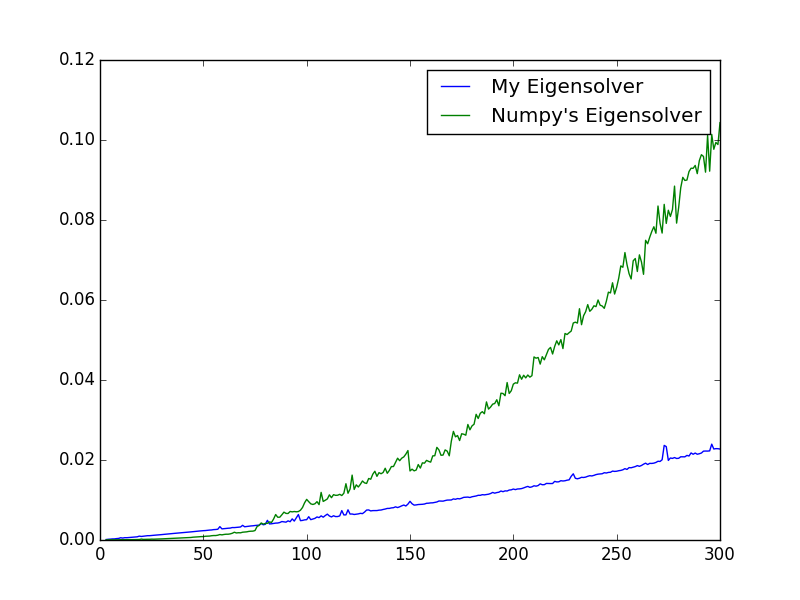
\includegraphics[width=\textwidth]{assets/graphics/figure_1.png}
\caption{Scaling to $n=300$}
\end{figure}

\vfill

\pagebreak

\subsection{Plotting the first few
eigenfunctions}\label{plotting-the-first-few-eigenfunctions}

\begin{Shaded}
\begin{Highlighting}[]
\KeywordTok{def} \NormalTok{for_plot_K_eigenfunction(k,n):}
  \NormalTok{vec }\OperatorTok{=} \NormalTok{K_eigenfunction(k,n)}
  \NormalTok{soln }\OperatorTok{=} \NormalTok{np.insert(vec,}\DecValTok{0}\NormalTok{,}\DecValTok{0}\NormalTok{)}
  \NormalTok{soln }\OperatorTok{=} \NormalTok{np.insert(np.zeros(}\DecValTok{1}\NormalTok{),}\DecValTok{0}\NormalTok{,soln)}
  \ControlFlowTok{return} \NormalTok{soln   }

\KeywordTok{def} \NormalTok{plot_m_K_eigenfunctions(m,n):}
  \ControlFlowTok{for} \NormalTok{i }\OperatorTok{in} \BuiltInTok{range}\NormalTok{(m}\DecValTok{+1}\NormalTok{):}
  \NormalTok{plt.plot(np.linspace(}\DecValTok{0}\NormalTok{,}\DecValTok{1}\NormalTok{,n}\DecValTok{+2}\NormalTok{),for_plot_K_eigenfunction(i,n))  }

\NormalTok{plot_m_K_eigenfunctions(}\DecValTok{4}\NormalTok{,}\DecValTok{10}\NormalTok{)}
\NormalTok{plot_m_K_eigenfunctions(}\DecValTok{4}\NormalTok{,}\DecValTok{20}\NormalTok{)}
\NormalTok{plot_m_K_eigenfunctions(}\DecValTok{4}\NormalTok{,}\DecValTok{1000}\NormalTok{)}
\end{Highlighting}
\end{Shaded}

\begin{figure}[htbp]
\centering
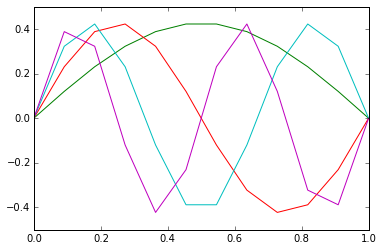
\includegraphics{assets/graphics/1_5_eigenvectors_23_1.png}
\caption{First four eigenfunctions, n=10}
\end{figure}

\begin{figure}[htbp]
\centering
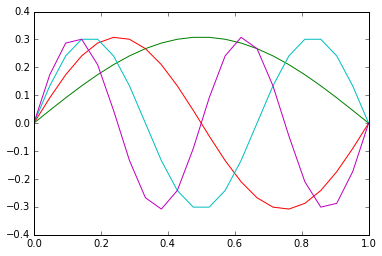
\includegraphics{assets/graphics/1_5_eigenvectors_24_1.png}
\caption{First four eigenfunctions, n=20}
\end{figure}

\begin{figure}[htbp]
\centering
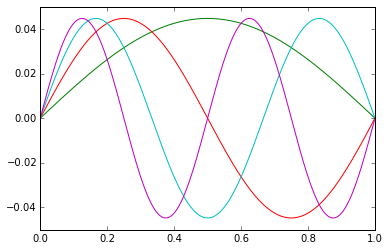
\includegraphics{assets/graphics/1_5_eigenvectors_25_1.png}
\caption{First four eigenfunctions, n=10000}
\end{figure}

\chapter{Power Method}\label{power-method}

\section{Solving Molecular Quantum Mechanics Problems
Computationally}\label{solving-molecular-quantum-mechanics-problems-computationally}

At its essence the work in Dr.~Eloranta's lab is an extension of the
simple power method for finding an eigenvector. Also known as the Von
Mises Iteration, the simple power method operates on a few well
conditionings, all of which are satisfied by our Hamiltonian matrices
--- namely we require self-adjoint matrices, and all that this implies.

The power method will only return the dominant eigenvector of an
operator. Essentially, the next vector in the iteration is calculated by
multiplying the current vector by the matrix being examined and then
normalizing.

\vfill

\pagebreak

\section{Simple Power Method}\label{simple-power-method}

\begin{enumerate}
\def\labelenumi{\arabic{enumi}.}
\item
  Choose a starting vector \(\mathbf{x}^{(0)}\in\mathcal{R}^n\) with
  \(\rvert\rvert\mathbf{x}^{(0)}\rvert\rvert=1\).
\item
  \(k=0\)
\item
  \texttt{while} some convergence criteria is not satisfied

  \begin{enumerate}
  \def\labelenumii{\roman{enumii}.}
  \tightlist
  \item
    \(k:=k+1\)
  \item
    \(\mathbf{y}^{(k)}:=A\mathbf{x}^{(k-1)}\)
  \item
    \(\mu_k:=\rvert\rvert\mathbf{y}^{(k)}\rvert\rvert\)
  \item
    \(\mathbf{x}^{(k)}:=\mathbf{y}^{(k)}/\mu_k\)
  \end{enumerate}
\end{enumerate}

The eigenvalue can be found by calculating

\begin{align*}
\lambda u &= A u\\
u^T\lambda u &= u^TA u\\
\lambda &= u^TAu \tag{because $u$ is normalized}
\end{align*}

\vfill

\pagebreak

Here we define an iteration and that iterate 100 times to find our the
eigenvector associated with the largest eigenvalue.

\begin{verbatim}
def power_iteration(A,u,n):
  for i in range(n):
    u      = A.dot(u)
    mu     = numpy.sqrt(u.dot(u))
    u      = u/mu
  eigvec = u
  eigval = eigval = u.dot(A.dot(u))
  return eigval, eigvec

In [1]: import numpy, scipy.linalg, numpy.random

In [2]: B = numpy.random.rand(4,4)

In [3]: C = B.dot(B.T) # returns a symmetric matrix

In [4]: y = numpy.random.rand(4)

In [5]: power_iteration(C,u,100)
Out[5]: (5.4509787314661642,
 array([ 0.57243721,  0.54380344,  0.38428034,  0.47845802]))

In [6]: scipy.linalg.eigh(C,eigvals=(3,3))
Out[6]:
(array([ 5.45097873]), 
 array([[-0.57243721],
        [-0.54380344],
        [-0.38428034],
        [-0.47845802]]))
\end{verbatim}

\subsection{Comparison of Timing}\label{comparison-of-timing-1}

\begin{verbatim}
In [7]: %timeit power_iteration(C,u,100)
1000 loops, best of 3: 351 µs per loop

In [8]: %timeit scipy.linalg.eigh(C,eigvals=(3,3))
The slowest run took 6.32 times longer than the fastest. 
This could mean that an intermediate result is being cached
10000 loops, best of 3: 26 µs per loop
\end{verbatim}

It is shown that our power iteration is considerably slower than the
built-in eigensolver. We are, however, hard coding the number of
iterations required.

\subsection{Stopping Criteria}\label{stopping-criteria}

It would behoove us to explore a better stopping criteria than simply
iterate 100 times. Toward this we propose the use of the norm of the
residual vector

\[\mathbf{r}=A\vecu^*-\lambda^*\vecu^*\]

We can then stop our calculation when
\(\rvert\rvert\mathbf r \rvert\rvert<\epsilon\) for any desired
\(\epsilon\).

\begin{verbatim}
def power_iteration(A,u,n,eps=0.00001):
  r_mag = 1
  while(r_mag > eps):
    u      = A.dot(u)
    mu     = numpy.sqrt(u.dot(u))
    u      = u/mu
    eigval = eigval = u.dot(A.dot(u))
    r      = A.dot(u)-eigval*u
    r_mag  = numpy.sqrt(r.dot(r))
  eigvec = u
  return eigval, eigvec

In [9]: %timeit power_iteration(C,u,100)
The slowest run took 6.79 times longer than the fastest. 
This could mean that an intermediate result is being cached
10000 loops, best of 3: 42.9 µs per loop
\end{verbatim}

While we are not beating the built-in solver, we are certainly within an
order of magnitude and are satisfied with these results.

\newcommand{\R}{\mathbb{R}}

\section{Iterative Techniques}\label{iterative-techniques}

\begin{description}
\item[vector norm]
a function from \(\R^n\) to \(\R\)

\(l_2\) norm is also called the Euclidean norm

\(\rvert\rvert \mathbf{x} \rvert\rvert_2 = \left(\sum_{i=1}^nx_i^2\right)^{1/2}\)
\item[convergence]
A sequence \(\left\{\mathbf{x}^{(k)}\right\}_{k=1}^\infty\) of vectors
in \(\R^n\) is said to converge to \(\mathbf{x}\) with respect to the
norm \(\rvert\rvert \cdot \rvert\rvert<\epsilon\), if given any
\(\epsilon>0\), there exists an integer \(N(\epsilon)\) such that

\[\rvert\rvert\mathbf{x}^{(k)}-\mathbf{x}\rvert\rvert<\epsilon
  \text{, for all }k\geq N(\epsilon)\]
\item[spectral radius]
the spectral radius of a matrix \(A\) is defined by

\[\rho(A)=\max\rvert\lambda\rvert|\]

where \(\lambda\) is an eigenvalue of \(A\).
\item[convergent matrices]
an \(n\) by \(n\) matrix is convergent if for all \(1\leq i,j \leq n\)

\[\lim_{k\to\infty}(A^k)_{ij}=0\]
\end{description}

\begin{Shaded}
\begin{Highlighting}[]

\end{Highlighting}
\end{Shaded}

\chapter{the Imaginary Time Propagation
Method}\label{the-imaginary-time-propagation-method}

\section{Applications of Imaginary Time Propagation Method in Material
Research}\label{applications-of-imaginary-time-propagation-method-in-material-research}

We are seeking approximate solutions to the time-independent Schrödinger
equation

\begin{align*}
H\Psi_i&=E_i\Psi_i\tag{eqn. 1}\\
\text{with }\hat{H}=\hat T + \hat V &= -\frac{\hbar^2}{2m}\Delta + V
\end{align*}

If we can find the eigenfunctions that satisfy these equations, the
corresponding eigenvalues can be found by calculating the expectation
value

\[\langle \psi_i \rvert H \rvert \psi_i \rangle\]

Our approach is the solve the time-dependent Schrödinger equation

\[i\hbar\frac{\partial}{\partial t}\Psi = \hat H \Psi\]

by converting it via a Wick rotation (let \(t=-i\tau\)) to a simple heat
equation:

\begin{align*}
\frac{\partial}{\partial t}\Psi=-\frac{\hat H}{\hbar}\Psi\tag{eqn. 2}
\end{align*}

Our solutions are then given by

\begin{align*}\Psi(r,t)=e^{-\hat H\tau/\hbar}\psi(r,0)=\left(e^{-\hat H\Delta\tau/\hbar}\right)^n\psi(r,0)\tag{eqn. 3}\end{align*}

Then \(\left(e^{-\hat H\Delta\tau/\hbar}\right)^n\) has the same
eigenfunctions as \(H\Psi_i=E_i\Psi_i\). If we iterate the decay
equation it will converge on the ground state.

We can solve eqn. 3 by treating it as an analog of the power method or
its generalization the subspace iteration.

As presented at NSF PREM Colloquium.

Helium droplets not only provide a unique matrix environment for high
resolution spec- troscopy and studying molecular solvation but also
allow to use guest molecules as probes of the surrounding quantum
medium.1--3 After the initial discovery of the helium droplet tech-
nique for spectroscopic applications, attention quickly turned into
characterizing the physical properties of the helium droplets
themselves. The groundbreaking experiments by the Toen-nies group
employed the glyoxal molecule as a probe to study the helium droplet
response through optical absorption spectrum.

\section{the Imaginary Time
Propagation}\label{the-imaginary-time-propagation}

The imaginary time propagation method (ITP) relies on solving the
time-dependent Schrödinger equation in imaginary time. We perform a Wick
Rotation (setting \(t=-i\tau\)) to transform the time-dependent
Schrödinger into a simple diffusion equation

\begin{equation}
\label{eq:itpSch}
\frac{\partial \psi(r,\tau)}{\partial
\tau}=-\frac{\hat{H}}{\hbar}\psi(r,\tau) \implies \psi(r,\tau)=\exp(-\hat{H}\tau/\hbar)\psi(r,0)
\end{equation}

\paragraph{Iterative Solutions to Eigenproblems}

This can be thought of as the analog to a power solution or subspace
iteration. As \(\tau\to\infty\), \(\psi(r,\tau)\) will converge on the
eigenfunction for the ground state.

In practice, a random vector is chosen as the initial state. A
time-propagation will yield the ground state eigenvector. If a vector
other than the ground state is desired, \(N\) separate wave functions
are propagated. Each higher state eigenvector is required to be
orthogonal to the lower eigenvectors and are thus discovered through the
iterative process. Approximate orthogonality is enforced in the
following way.

\begin{equation}
\label{eq:appxOrth}
\frac{\partial\psi_i(r,\tau)}{\partial\tau} = -\frac{\hat{H}}{\hbar}\psi(r,\tau)-\lambda\sum_{j < i}^N \rvert\langle \psi_j(r,\tau)\rvert\psi_i(r,\tau)\rangle\rvert^2
\end{equation}

\paragraph{}

In order to implement the solution computationally, the exponential
operator is approximated using the Cayley unitary form, transforming the
eigenvalue problem into a linear problem:

\begin{align*}
\label{eq:CayleyExpansion}
\exp(-H\Delta\tau)\approx\left(1+\frac{1}{2}H\Delta\tau\right)^{-1}\left(1-\frac{1}{2}H\Delta\tau\right) \\ 
\implies \left(1+\frac{1}{2}H\Delta\tau\right)\psi(r,\tau+\Delta\tau)=\left(1-\frac{1}{2}H\Delta\tau\right)\psi(r,\tau)
\end{align*}

\paragraph{Stopping Criteria}

A formula for the absolute error, \(\Delta E_i\) present in
\(E_i(\tau)\) can be written in terms of the quantum mechanical standard
deviation of \(H\) and is used as a stopping criteria.

\begin{equation}
\label{eq:error}
\Delta E_i = \rvert E_i -\langle\psi_i(r,\tau)\rvert H\rvert\psi_i(r,\tau)\rvert\leq\sqrt{2}\sqrt{\langle\psi_i(r,\tau)\rvert H^2\rvert\psi_i(r,\tau)\rangle-\langle\psi_i(r,\tau)\rvert H\rvert\psi_i(r,\tau)\rangle^2}
\end{equation}

\section*{Results}

The ITP method reduces the solving of an eigenproblem to an iterative
power solution via the solution of a linear equation. \% ITP is being
implemented in practice parallelized, using C and openBLAS. In current
practice has been shown to have better scalability than the implicitly
restarted Lanczos method as implemented in ARPACK.

For the purposes of training, the algorithm is being reimplemented in
Python and Numpy/Scipy. The solution of the linear equation being the
most computationally expensive, theoretically involving a matrix
inversion at each iteration, seven linear solution schemes were
speed-tested versus Numpy's built-in eigensolver: the Numpy solver, the
Scipy solver, Scipy's conjugate gradient squared (CGS) solver, a
Cholevsky decomposition method, two of Scipy's sparse solvers, and a
pre-inversion of the matrix iterated.

\begin{figure}[htbp]
\centering
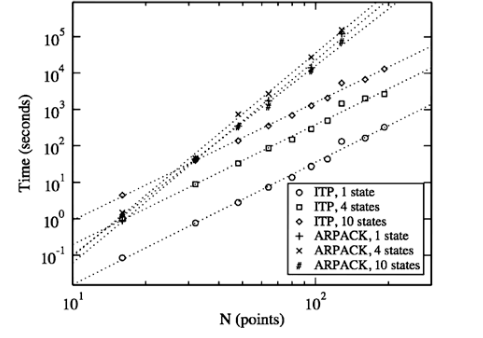
\includegraphics{assets/graphics/itpvlanc.png}
\caption{Computational scaling of the ITP and implicitly restarted
Lanczos methods (ARPACK) for 1, 4 and 10 states.}
\end{figure}

\begin{figure}[htbp]
\centering
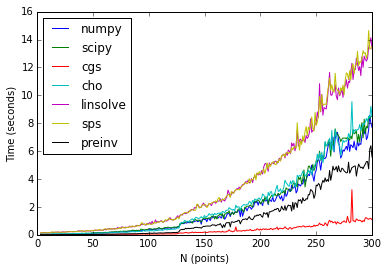
\includegraphics{assets/graphics/analysis_9_1.png}
\caption{Implementation of seven linear solving schemes in Python.}
\end{figure}

\begin{figure}[htbp]
\centering
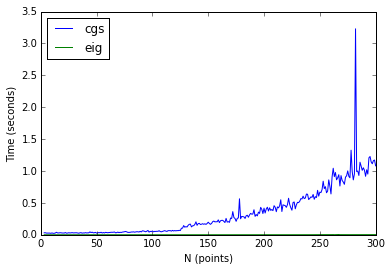
\includegraphics{assets/graphics/analysis_10_1.png}
\caption{Conjugate Gradient Squared Solver ITP v Built-in Eigensolver}
\end{figure}

The CGS solver was found to be the fastest. In comparison to the
built-in eigensolver, however, it falls well short of reasonable
performance standards. Furthermore, the CGS method has been found to be
the least stable of the methods (note the spike at \(N\approx 280\)).

\pagebreak

\section*{Applications to Bosonic Density Functional Theory}

Helium clusters were modeled by the Orsay-Trento DFT (OT-DFT) and the
interaction with the guest molecule was included through an external
potential. To compute the effective moment of inertia of the
molecule--helium complex, we include an additional energy term of the
form \(-\omega L_z\) and compute the ``rotating'' groundstate energy by
minimizing

\begin{equation}
\label{eq:OTDFT}
E[\Psi,\omega]=\int\left\{\frac{\hbar^2}{2m}\rvert\nabla\Psi\rvert^2+\epsilon_{OT}[\Psi]+V_{X-\text{He}}\rvert\Psi\rvert^2-\omega \Psi*L_z\Psi\right\}
\end{equation}

The non-linear Schrödinger-type equation arising from the minimization
of eq. 4 is solved by means of imaginary time propagation.

\section*{Bosonic Density Functional Theory}

In the experiment, bosonic density functional theory (DFT) is the method
used to obtain calculated rotational constant values. Density functional
theory is a technique that plays an important role in determining the
key components that can explain why the moment of inertia decreases when
rotational superfluidity takes place. The results obtained using DFT are
compared with experimental data and Quantum Monte Carlo (QMC) values and
there is a similar agreement which is shown by the appearance firs-turn
over point.

The first minimum appearing in molecular rotational constants as a
function of helium droplet size has been previously associated with the
onset of superfluidity in these finite systems. We investigate this
relationship by bosonic density functional theory calculations of
classical molecular rotors (OCS, N2O, CO and HCN) interacting with the
surrounding helium. The calculated rotational constants are in fair
agreement with the existing experimental data, demonstrating the
applicability of the theoretical model. By inspecting the spatial
evolution of the global phase and density, the increase in the
rotational constant after the first minimum is shown to correlate with
continuous coverage of the molecule by helium and appearance of angular
phase coherence rather than completion of the first solvent shell. We
assign the observed phenomenon to quantum phase transition between a
localized state and one-dimensional superfluid, which represents the
onset of rotational superfluidity in small helium droplets.

\begin{Shaded}
\begin{Highlighting}[]

\end{Highlighting}
\end{Shaded}

\appendix

\chapter{Appendix}\label{appendix}

\section{Structuring a Scientific
Project}\label{structuring-a-scientific-project}

The below are important highlights from
\href{http://journals.plos.org/ploscompbiol/article?id=10.1371/journal.pcbi.1000424\#pcbi-1000424-g001}{\emph{A
Quick Guide to Organizing Computational Biology Projects}} by William
Noble.

\begin{quote}
It is generally a good idea to store all of the files relevant to one
project under a common root directory.
\end{quote}

\begin{quote}
use a top-level organization that is logical, with chronological
organization at the next level, and logical organization below that
\end{quote}

\begin{figure}
\fbox{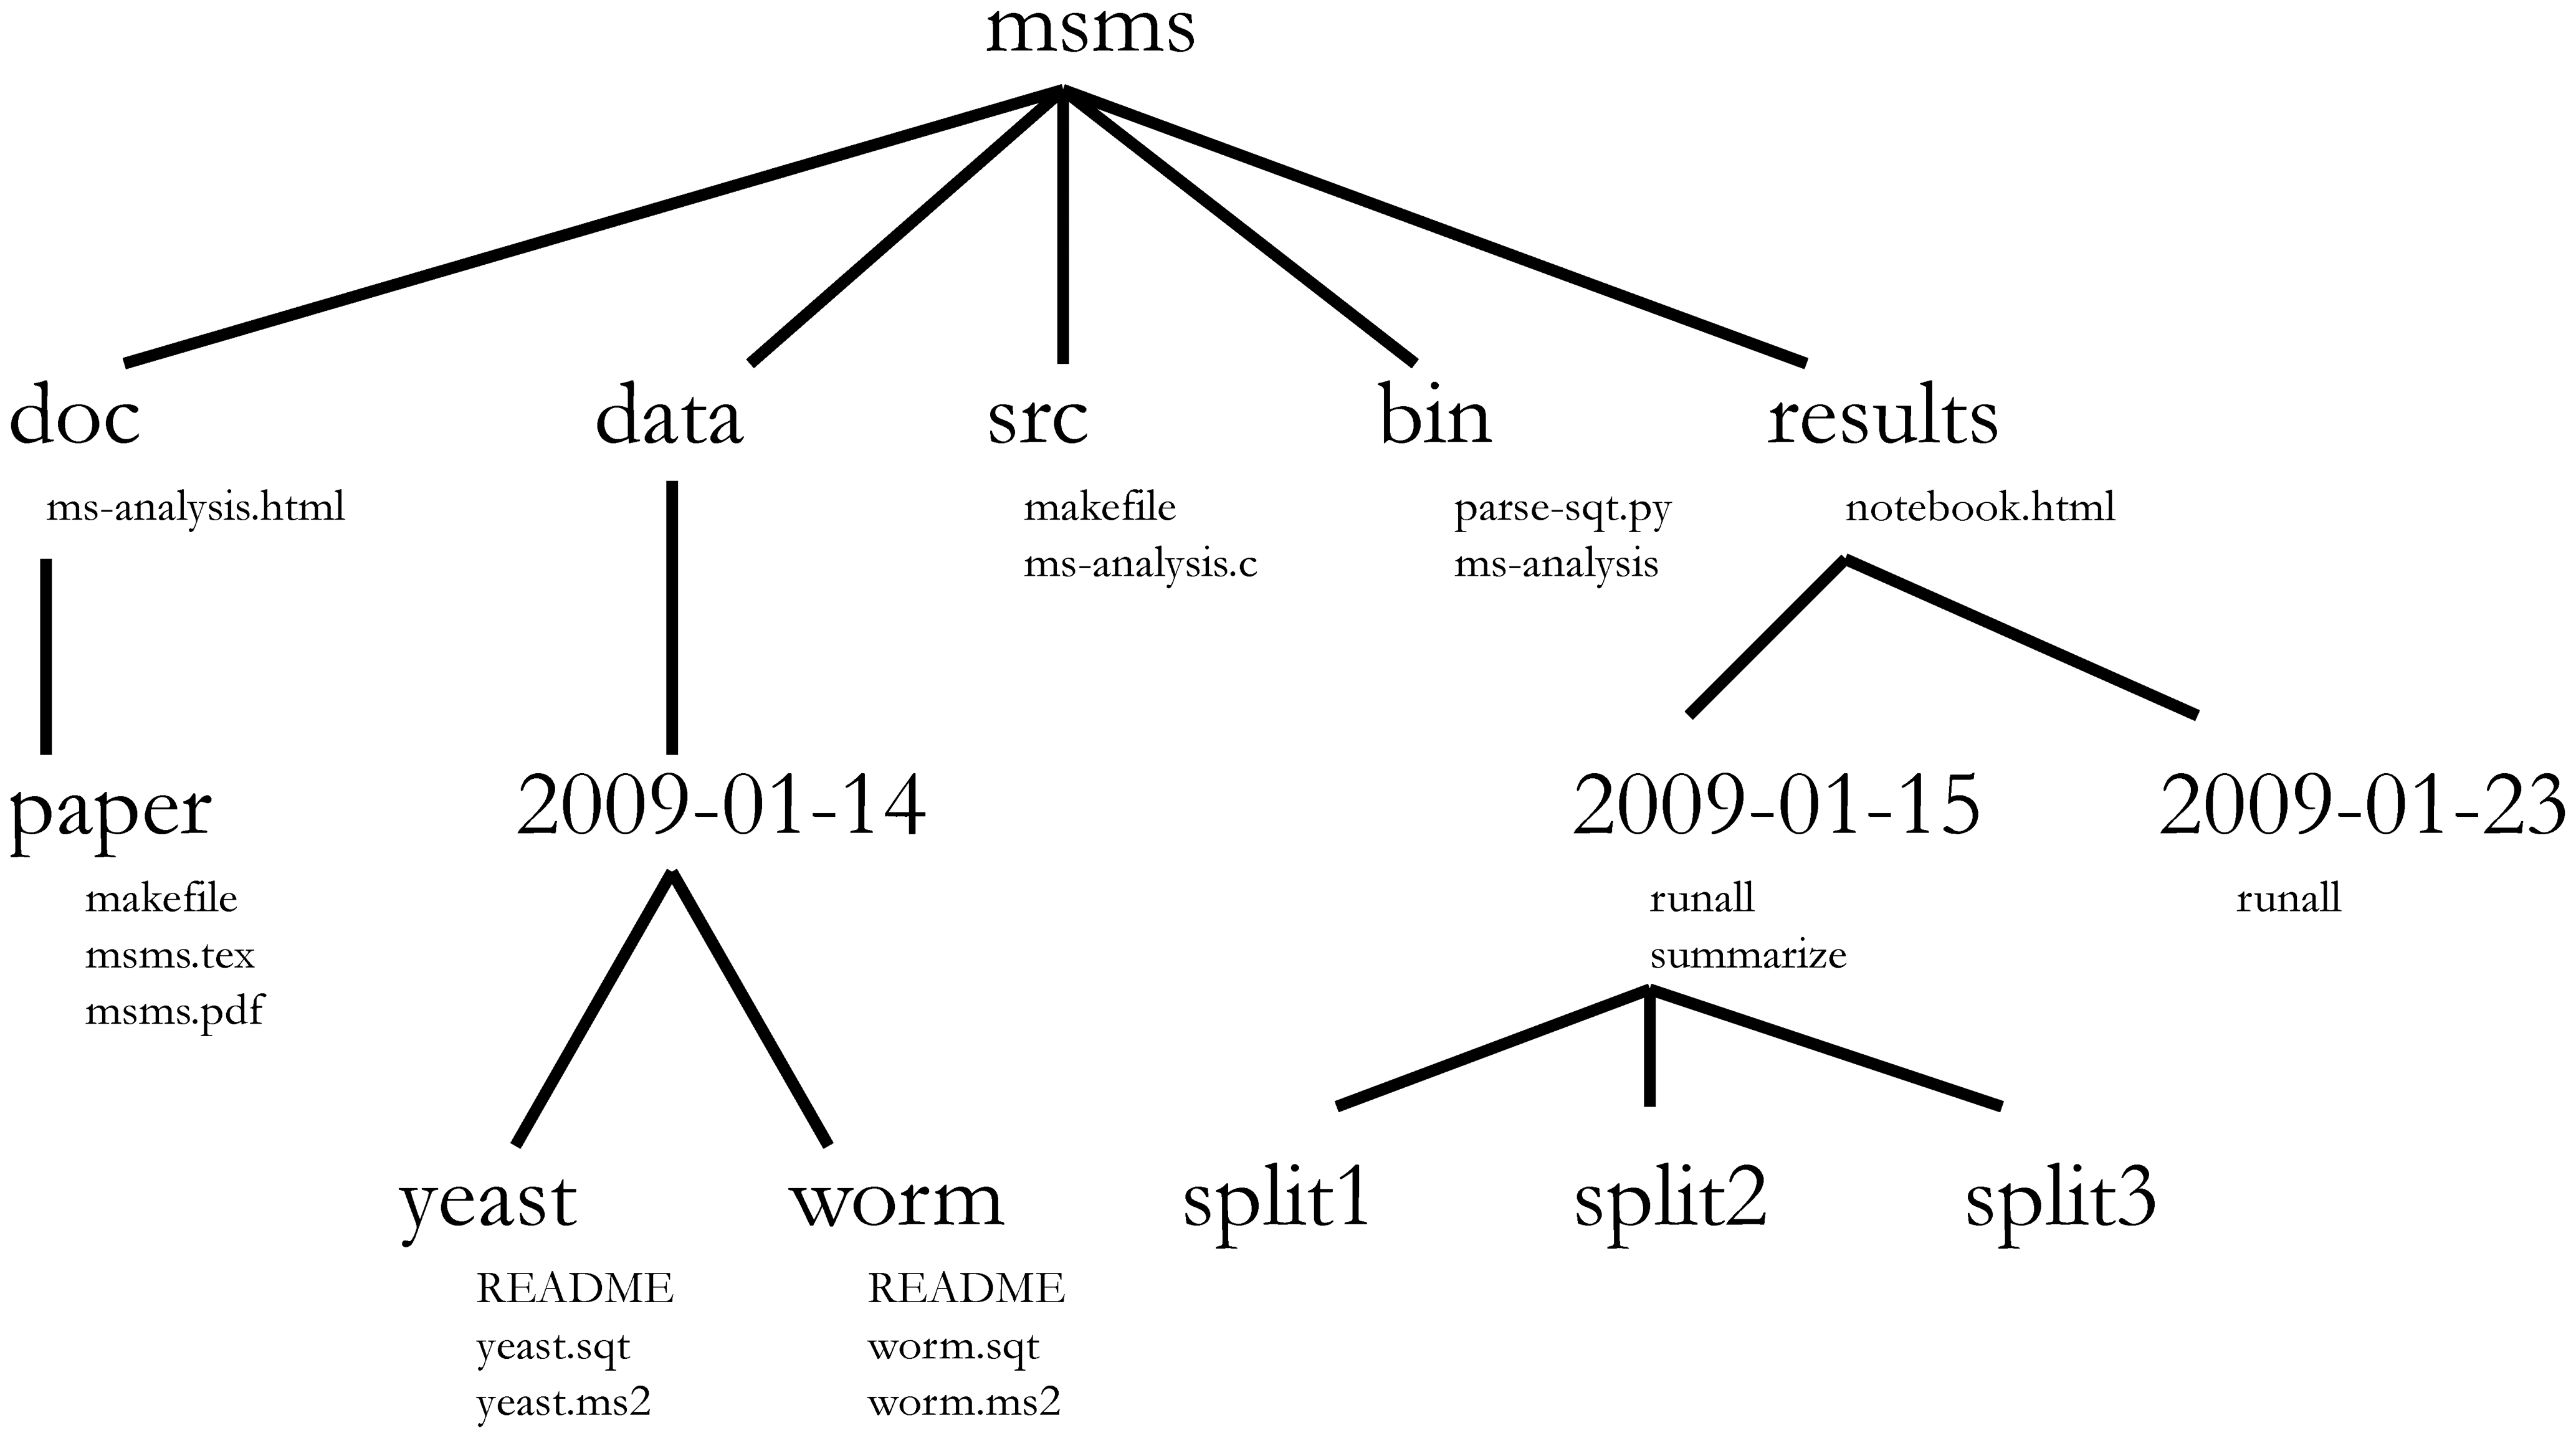
\includegraphics[width=1\linewidth]{assets/graphics/journal-pcbi-1000424-g001.png}}
\caption{Structuring a Scientific Project}
\end{figure}

\begin{quote}
In parallel with this chronological directory structure, I find it
useful to maintain a chronologically organized lab notebook. This is a
document that resides in the root of the results directory and that
records your progress in detail. Entries in the notebook should be
dated, and they should be relatively verbose, with links or embedded
images or tables displaying the results of the experiments that you
performed.
\end{quote}

\subsection{Carrying Out a Single
Experiment}\label{carrying-out-a-single-experiment}

\begin{quote}
record every operation that you perform
\end{quote}

\begin{quote}
create either a README file, in which I store every command line that I
used while performing the experi- ment, or a driver script (I usually
call this runall) that carries out the entire exper- iment automatically
\end{quote}

\begin{quote}
I work in a combination of shell scripts, Python, and C
\end{quote}

\begin{quote}
Whatever you decide, you should end up with a file that is parallel to
the lab notebook entry
\end{quote}

\begin{quote}
Here are some rules of thumb that I try to follow when developing the
driver script:
\end{quote}

\begin{quote}
\begin{enumerate}
\def\labelenumi{\arabic{enumi}.}
\tightlist
\item
  Record every operation that you per- form.
\end{enumerate}
\end{quote}

\begin{quote}
\begin{enumerate}
\def\labelenumi{\arabic{enumi}.}
\setcounter{enumi}{1}
\tightlist
\item
  Comment generously.
\end{enumerate}
\end{quote}

\begin{quote}
\begin{enumerate}
\def\labelenumi{\arabic{enumi}.}
\setcounter{enumi}{2}
\tightlist
\item
  Avoid editing intermediate files by hand.
\end{enumerate}
\end{quote}

\begin{quote}
Many simple editing opera- tions can be performed using standard Unix
utilities such as sed, awk, grep, head, tail, sort, cut, and paste.
\end{quote}

\begin{quote}
\begin{enumerate}
\def\labelenumi{\arabic{enumi}.}
\setcounter{enumi}{3}
\tightlist
\item
  Store all file and directory names in this script.
\end{enumerate}
\end{quote}

\begin{quote}
\begin{enumerate}
\def\labelenumi{\arabic{enumi}.}
\setcounter{enumi}{4}
\tightlist
\item
  Use relative pathnames to access other files within the same project.
\end{enumerate}
\end{quote}

\begin{quote}
\begin{enumerate}
\def\labelenumi{\arabic{enumi}.}
\setcounter{enumi}{5}
\tightlist
\item
  Make the script restartable.
\end{enumerate}
\end{quote}

\begin{quote}
For experiments that take a long time to run, I find it useful to be
able to obtain a summary of the experiment's progress thus far.
\end{quote}

\subsection{Command Lines versus Scripts versus
Programs}\label{command-lines-versus-scripts-versus-programs}

\begin{quote}
\begin{enumerate}
\def\labelenumi{\arabic{enumi}.}
\tightlist
\item
  Driver Script
\end{enumerate}
\end{quote}

\begin{quote}
\begin{enumerate}
\def\labelenumi{\arabic{enumi}.}
\setcounter{enumi}{1}
\tightlist
\item
  Single-use Script
\end{enumerate}
\end{quote}

\begin{quote}
\begin{enumerate}
\def\labelenumi{\arabic{enumi}.}
\setcounter{enumi}{2}
\tightlist
\item
  Project-specific script
\end{enumerate}
\end{quote}

\begin{quote}
\begin{enumerate}
\def\labelenumi{\arabic{enumi}.}
\setcounter{enumi}{3}
\tightlist
\item
  Multi-project script.
\end{enumerate}
\end{quote}

\begin{quote}
Regardless of how general a script is supposed to be, it should have a
clearly documented interface.
\end{quote}

\subsection{The Value of Version
Control}\label{the-value-of-version-control}

\begin{quote}
provides a form of backup
\end{quote}

\begin{quote}
version control provides a historical record that can be useful for
tracking down bugs or understanding old results.
\end{quote}

\begin{quote}
invaluable for collaborative projects
\end{quote}

\begin{quote}
changes should be checked in at least once a day
\end{quote}

\begin{quote}
it is possible to check in your changes on a ``branch'' of the project
\end{quote}

\begin{quote}
should only be used for files that you edit by hand
\end{quote}

\begin{Shaded}
\begin{Highlighting}[]

\end{Highlighting}
\end{Shaded}

\section{Glossary}\label{glossary}

\begin{description}
\tightlist
\item[Adjoint]
rises in many fields of mathematics. It can be defined in
infinite-dimensional complex scalar product spaces (finite-dimensional
case).
\item[Boundary Conditions]
\item[Classical Mechanics]
no limitations in the accuracy with which observables may be measured.
\item[Complete Basis Set]
In a particular space a list of vectors or functions that is linearly
independent and spans the space.
\item[Continuous]
A set of data is said to be continuous if the values belonging to the
set can take on ANY value within a finite or infinite interval. Some
examples in quantum mechanics are position and momentum.
\item[Difference Matrix]
\item[Differentiable]
\item[Differential Operator]
\item[Discrete]
A set of data is said to be discrete if the values belonging to the set
are distinct and separate (unconnected values). An example in quantum
mechanics is spin states.
\item[Eigenequation]
a relationship describing a vector or function that is invariant with
respect to a given linear operator. Given an operator
\(\Gamma: \mathbb{F}^n \to \mathbb{F}^n\), where \(\mathbb{F}^n\)
represents either the Real or Complex field of dimenion \(n\),
\(\Gamma\) is said to be in the set of linear operators over the space
\(\mathbb{F}^n\). Then, \(\lambda\) and \(\psi\) are said to be an
eigenvalue and eigenvector respectively of the linear operator
\(\Gamma\), if \(\lambda\in\mathbb{F}\), \(\psi\neq0\) and
\(\Gamma\psi=\lambda\psi\) ({[}@eq:eigenequation{]})
\item[Eigenfunction]
\item[Eigenvector]
it's a measurable quantity known as observables in quantum mechanics.
\item[Eigenvalue]
if we are given the following equation: , then the eigenvalue of an
operator is .
\item[Energy]
the sum of potential and kinetic energies where is kinetic energy and is
potential energy.
\item[Hamiltonian Operator]
Classically, the Hamiltonian corresponds to the total energy of a
system. The Hamiltonian operator is the corresponding quantum mechanical
operator and is equal to the sum of the kinetic and potential energy
operators.

\(H=T+V=-\frac{\hbar^2}{2m}\nabla^2 + V\)
({[}@eq:definition\_hamiltonian{]})

The expectation value of the Hamiltonian operator is an associated
energy, \(E\) that is totally conserved.
\item[Invertible]
\item[Kinetic Energy]
\item[Linear Combination]
Given a complete set of basis functions, it is possible to write a
wavefunction describing the state of a system as a linear combination of
this basis set. In other words,
\(\psi(\mathbf{r})=\sum_{i=1}^\infty c_i\phi_i\)\$
({[}@eq:linear\_combination{]}), where \(\Gamma \phi_i = a_i\phi_i\).
\item[Linear Operator]
\item[Observable]
any dynamical variable that can be measured.
\item[Planck's Constant]
\item[Positive Definite]
\item[Potential Energy]
\item[Probability]
\item[Quantum Mechanics]
\item[Schrödinger's Equation]
Time-Dependent is

\textbf{Time-Independent} \(H\psi=E\psi\)
({[}@eq:time\_independent\_schrodinger{]})
\item[Self-Adjoint Linear Operator]
The adjoint of a linear operator \(L\) is the unique linear operator
\(L^*\) that satisfies

\(\llangle L[u],v\rrangle = \langle u,L^*v\rangle\) ({[}@eq:adjoint{]})

An operator is called self-adjoint if \(L=L^*\). For a self-adjoint
operator, the eigenvalues are real and the eigenvectors are orthogonal.
\item[Sparse]
\item[Spectral Theory]
\item[State]
\item[Steady-State]
\item[Symmetric Matrix]
\item[System]
\item[Tridiagonal]
\item[Vector]
\item[Wave Function]
\end{description}

\begin{Shaded}
\begin{Highlighting}[]

\end{Highlighting}
\end{Shaded}

\section{C}\label{c}

\paragraph{GSL}

Central to this work is the \href{http://www.gnu.org/software/gsl/}{GNU
Scientific Library} which offers implementations of \texttt{openblas}
(Open Basic Linear Algebra System) and \texttt{lapack} (Linear Algebra
Package) necessary for the completion of this work. We have used
\texttt{homebrew} to install \texttt{gsl} and \texttt{pkg-config}

\begin{verbatim}
$ brew install pkg-config
$ brew install gsl
$ pkg-config --libs gsl
-L/usr/local/Cellar/gsl/1.16/lib -lgsl -lgslcblas -lm
\end{verbatim}

and then added the linker statements to our makefile:

\begin{verbatim}
#Tool Definitions
CC=gcc
CFLAGS=-I. -I$(PATHU) -DTEST
CFLAGS+=-I/usr/local/opt/openblas/include
CFLAGS+=-lgsl -lgslcblas -lm
\end{verbatim}

\paragraph{Known Eigenvalues}

We have written a short python script in order to calculate a few known
eigenvalues, in this case for the 4th order Hibert Matrix.

\begin{verbatim}
import numpy
import scipy
from scipy.linalg import *

h4 = hilbert(4)
eigs_h4 = eig(h4)
print eigs_h4
\end{verbatim}

\paragraph{Test-Driven Development}

We begin the project with a simple tests to verify the known eigenvalues
we have previously generated.

\begin{verbatim}
#include <stdio.h>
#include <math.h>
#include <gsl/gsl_math.h>
#include <gsl/gsl_eigen.h>
#include "minunit.h"

#define DIMENSION_OF(a) (sizeof(a)/sizeof(a[0]))

gsl_vector * symmetric_eigenvalues(double * data, int return_values);

float round_to_5_places(float num);

int tests_run = 0;

double expected_eigenvalues[] = {1.500214,0.169141,0.006738,0.000097};

double fourth_order_hilbert[] =
{
  1.0  , 1/2.0, 1/3.0, 1/4.0,
  1/2.0, 1/3.0, 1/4.0, 1/5.0,
  1/3.0, 1/4.0, 1/5.0, 1/6.0,
  1/4.0, 1/5.0, 1/6.0, 1/7.0
};

static char * test_find_eigenvalues()
{
  gsl_vector * actual_eigenvalues = symmetric_eigenvalues(fourth_order_hilbert,0);

  for (int i = 0; i < DIMENSION_OF(expected_eigenvalues); i++)
  {
     float expected = expected_eigenvalues[i];
     float actual = round_to_5_places(gsl_vector_get(actual_eigenvalues, i));

     printf("\nexpected: %f actual: %f\n",
       expected,actual);
     mu_assert("error, eigenvalues do not match",
         expected == actual);
  }
  return 0;
}

static char * all_tests()
{
  mu_run_test(test_find_eigenvalues);
  return 0;
}

int main(int argc, char **argv)
{
  char * result = all_tests();
  if (result != 0)
  {
    printf("%s\n", result);
  }
  else
  {
    printf("All Tests Passed\n");
  }
  printf("Tests run: %d\n", tests_run);

  return result != 0;
}

gsl_vector * symmetric_eigenvalues(double * data, int return_values)
{
  gsl_matrix_view my_matrix = gsl_matrix_view_array (data, 4, 4);

  gsl_vector * my_evals = gsl_vector_alloc (4);
  gsl_matrix * my_evecs = gsl_matrix_alloc (4, 4);

  gsl_eigen_symmv_workspace * my_workspace = gsl_eigen_symmv_alloc (4);

  gsl_eigen_symmv (&my_matrix.matrix, my_evals, my_evecs, my_workspace);

  gsl_eigen_symmv_free (my_workspace);

  gsl_eigen_symmv_sort (my_evals, my_evecs, GSL_EIGEN_SORT_ABS_DESC);

  return my_evals;
}

float round_to_5_places(float num)
{
  float nearest = roundf(num * 1000000) / 1000000;
  return nearest;
}
\end{verbatim}

\paragraph{Comments and Further Consideration}

I am not pleased with this particular test of the Symmetic Eigensolver
implemented in GSL. It is very ``numerical''. I think a better test
would be more mathematical, such as a test of any matrix and the
eigenequation itself, \(Ax=\lambda x\). I did, however, confirm that
MinUnit is an excellent way to begin to implement a TDD mindset in C
development. I think that the next step is to begin to write more tests
around the openBlas implementation in the GSL.

\paragraph{MinUnit}

As per MinUnit's description, ``MinUnit is an extremely simple unit
testing framework written in C. It uses no memory allocation, so it
should work fine under almost any circumstance, including ROMable
code.''

\begin{verbatim}
/* file: minunit.h */
 #define mu_assert(message, test) do { if (!(test)) return message; } while (0)
 #define mu_run_test(test) do { char *message = test(); tests_run++; \
                                if (message) return message; } while (0)
 extern int tests_run;
\end{verbatim}

As per MinUnit's description: ``No, that's not a typo. It's just 3 lines
of code.''

MinUnit has also been added to \texttt{tools}.

I wanted to be able to add more information to tests being run using the
\href{http://www.jera.com/techinfo/jtns/jtn002.html}{\texttt{minunit.h}}
testing harness. In particular, I wanted to think of a test run as a
``test'' and an individual assert within that test run as a subtest. I
wanted to be able to name each of these and have their status displayed
in \texttt{STDOUT}.

\paragraph{My MinUnit Implementation}

\begin{verbatim}
/* file: my_minunit.h */
#define mu_assert(subtest_desc, test,message) do { \
   if (!(test)) { \
   printf("subtest: \"%s\" FAILED\n", subtest_desc); \
   return message; \
   } \
   else { \
     printf("subtest: \"%s\" PASSED\n", subtest_desc); \
   } \
} while (0)

#define mu_run_test(test_desc,test) do { \
  printf("\nTest: \"%s\"\n",test_desc); \
  char *message = test(); tests_run++; \
  if (message) return message; } while (0)

extern int tests_run;
\end{verbatim}

A little less minimal but still small. I also added this file to
\texttt{/usr/include} so as to not have to tell \texttt{gcc} where to
find it.

\paragraph{A typical output}

\begin{verbatim}

Test: "Test of GSL"
y: -0.177597     expected_y: -0.177597
subtest: "value of zero order Bessel function of the first kind" PASSED

Test: "Test of Rectangular Complex Number Struct"
subtest: "real part of a rectangular complex number" PASSED
subtest: "imaginary part of a rectangular complex number" PASSED
subtest: "real part of a rectangular complex number after redefinition" PASSED
subtest: "imaginary part of a rectangular complex number after redefinition" PASSED

All Tests Passed
Tests run: 2
\end{verbatim}

\paragraph{Spec file for this output}

\begin{verbatim}
#include <stdio.h>
#include <gsl/gsl_sf_bessel.h>
#include <gsl/gsl_complex_math.h>
#include <math.h>
#include <my_minunit.h>

int tests_run = 0;
float round_to_6_places(float num);

static 
char * test_gsl_via_0_order_bessel_function_of_the_first_kind ()
{
  double x = 5.0;
  double y = round_to_6_places(gsl_sf_bessel_J0 (x));
  double expected_y = round_to_6_places(-1.775967713143382920e-01);
  printf("y: %f \t expected_y: %f\n",y,expected_y);
  mu_assert
  (
    "value of zero order Bessel function of the first kind",
    y == expected_y,
    "y: not equal to expected_y" 
  );
  return 0;
}

static
char * test_gsl_rectangular_complex_number_struct()
{
  double x = 2.43728;
  double y = 3.23412;

  gsl_complex test_rect_complex_number = gsl_complex_rect ( x, y ); 

  mu_assert
  (
    "real part of a rectangular complex number",
    GSL_REAL(test_rect_complex_number) == x,
    "real part of rectangular complex number does not match expected" 
  );

  mu_assert
  (
    "imaginary part of a rectangular complex number",
    GSL_IMAG(test_rect_complex_number) == y,
    "imaginary part of rectangular complex number does not match expected" 
  );

  GSL_SET_REAL(&test_rect_complex_number,y);
  GSL_SET_IMAG(&test_rect_complex_number,x);
  
  mu_assert
  (
    "real part of a rectangular complex number after redefinition",
    GSL_REAL(test_rect_complex_number) == y,
    "redefined real part of rectangular complex number does not match expected" 
  );

  mu_assert
  (
    "imaginary part of a rectangular complex number after redefinition",
    GSL_IMAG(test_rect_complex_number) == x,
    "redefined imaginary part of rectangular complex number does not match expected" 
  );

  return 0;
}  

static 
char * all_tests ()
{
  mu_run_test("Test of GSL", test_gsl_via_0_order_bessel_function_of_the_first_kind); 
  mu_run_test("Test of Rectangular Complex Number Struct", 
              test_gsl_rectangular_complex_number_struct);
  return 0;
}

int 
main(int argc, char **argv)
{
  char * result = all_tests();
  if (result != 0)
  {
    printf("%s\n", result);
  }
  else
  {
    printf("\nAll Tests Passed\n");
  }
  printf("Tests run: %d\n", tests_run);

  return result != 0;
}

float 
round_to_6_places(float num)
{
  float nearest = roundf(num * 10000000) / 10000000;
  return nearest;
}
\end{verbatim}

\section{Python}\label{python}

While Python comes preinstalled with Mac OS X, installing through
homebrew ensures that you have the most updated version as well as moves
the management of Python to homebrew.

\begin{verbatim}
brew install python 
\end{verbatim}

Python comes installed by default, but best to get the latest and
greatest.

The above installs \texttt{pip}.

\paragraph{Install Basic Python Packages}

Most of the pip installs require that they be run as \texttt{sudo}.
\texttt{brew} is not a fan of \texttt{sudo} and should not have the same
requirements.

\begin{verbatim}
pip install numpy
pip install scipy
pip install matplotlib
\end{verbatim}

\paragraph{Python as a Tool for Developing C Algorithms}

emulating minunit in python {[}{[}Needs Work{]}{]}

\paragraph{IPython}

\begin{verbatim}
pip install ipython
\end{verbatim}

This did not install all of the dependencies required to run IPython
notebook. It was fairly straightforward to identify the missing
dependencies, however, by attempting to run \texttt{IPython\ Notebook}.

\begin{verbatim}
ipython notebook 
\end{verbatim}

The following three dependencies were succesively required:

\begin{verbatim}
pip install pyzmqi
pip install jinjaz
pip install tornado
\end{verbatim}

\paragraph{Numpy}

\paragraph{Scipy}

\paragraph{Fabric}

\section{Unix-Like}\label{unix-like}

\paragraph{Pandoc}

If you need to convert files from one markup format into another, pandoc
is your swiss-army knife.
\href{http://johnmacfarlane.net/pandoc/}{Pandoc} can convert documents
in markdown, reStructuredText, textile, HTML, DocBook, LaTeX, MediaWiki
markup, TWiki markup, OPML, Emacs Org-Mode, Txt2Tags, Microsoft Word
docx, EPUB, or Haddock markup to

\begin{itemize}
\tightlist
\item
  HTML formats: XHTML, HTML5, and HTML slide shows using Slidy,
  reveal.js, Slideous, S5, or DZSlides.
\item
  Word processor formats: Microsoft Word docx, OpenOffice/LibreOffice
  ODT, OpenDocument XML
\item
  Ebooks: EPUB version 2 or 3, FictionBook2
\item
  Documentation formats: DocBook, GNU TexInfo, Groff man pages, Haddock
  markup
\item
  Page layout formats: InDesign ICML
\item
  Outline formats: OPML
\item
  TeX formats: LaTeX, ConTeXt, LaTeX Beamer slides
\item
  PDF via LaTeX
\item
  Lightweight markup formats: Markdown, reStructuredText, AsciiDoc,
  MediaWiki markup, DokuWiki markup, Emacs Org-Mode, Textile
\item
  Custom formats: custom writers can be written in lua.
\end{itemize}

Pandoc was (and is) used to render ``final'' pdfs of the work done.
Pandoc files were written in a hybrid of markdown (for document
formatting) and Latex (for math rendering) that mirror the presentation
format of IPython Notebooks.

\paragraph{Install Pandoc}

\begin{verbatim}
brew install pandoc
\end{verbatim}

You will need a reasonably robust \LaTeX installation.

\begin{Shaded}
\begin{Highlighting}[]

\end{Highlighting}
\end{Shaded}

\section{docker}\label{docker}

\subsection{Best practices in writing a
Dockerfile}\label{best-practices-in-writing-a-dockerfile}

https://docs.docker.com/engine/userguide/eng-image/dockerfile\_best-practices/

https://github.com/dockerfile/mongodb/blob/master/Dockerfile

https://github.com/jupyter/docker-stacks/blob/master/datascience-notebook/Dockerfile

\begin{Shaded}
\begin{Highlighting}[]

\end{Highlighting}
\end{Shaded}

\end{document}
